\documentclass[11pt,a4paper]{book}

\usepackage{lib/Textbook}
\exhyphenpenalty=10000\hyphenpenalty=10000
%\sloppy
\usepackage{enumitem}
\usepackage{mdframed}
\usepackage{tikz}
\usepackage{nccmath}
\usepackage{wrapfig}
\usepackage{textcomp}
\usepackage{multirow}
\usepackage{tasks}
\usetikzlibrary{shapes,arrows,decorations.pathreplacing,calc,positioning,intersections}
\usepackage[export]{adjustbox}
\usepackage{chngcntr}
\usepackage{array}
\usepackage{picture}
\tikzstyle{Box} = [rectangle, minimum height=1cm, draw=black]
\tikzstyle{arrow} = [thick, ->, >=stealth]

\newlist{steps}{enumerate}{1}
\setlist[steps, 1]{label = Step \arabic*:}

\newlist{inlinelist}{enumerate*}{1}
\setlist[inlinelist]{itemjoin = \hspace{.5in}, label=(\alph*)}

\newcommand{\R}{\mathbb{R}}
\newcommand{\N}{\mathbb{N}}
\newcommand{\Z}{\mathbb{Z}}
\newcommand{\Q}{\mathbb{Q}}
\newcommand{\W}{\mathbb{W}}
\newcommand{\C}{\mathbb{C}}

\usepackage{ulem}
\usepackage{graphicx}

\usepackage[english]{babel}
\usepackage{lipsum}
\usepackage{xcolor}
\usepackage{tikz}
\usepackage{mathtools,amsfonts,amssymb,amsthm}
\usepackage[most]{tcolorbox}
\usepackage{cancel}
\setlength{\parindent}{0pt}

\usepackage{fourier}

\makeatletter
\newcommand*\bigcdot{\mathpalette\bigcdot@{.5}}
\newcommand*\bigcdot@[2]{\mathbin{\vcenter{\hbox{\scalebox{#2}{$\m@th#1\bullet$}}}}}
\makeatother

\makeatletter
\newcommand{\newparallel}{\mathrel{\mathpalette\new@parallel\relax}}
\newcommand{\new@parallel}[2]{%
  \begingroup
  \sbox\z@{$#1T$}% get the height of an uppercase letter
  \resizebox{!}{\ht\z@}{\raisebox{\depth}{$\m@th#1/\mkern-5mu/$}}%
  \endgroup
}
\makeatother


% Von Koch Snowflake

\usetikzlibrary{lindenmayersystems}


\tikzset{
  Koch curve/.style = {
    l-system={
      rule set={F -> F-F++F-F},
      axiom=F++F++F,
      step=1pt,
      angle=60,
      #1
    }
  }
}


\let\cleardoublepage=\clearpage


% Start document
\begin{document}

\tableofcontents
\chapter{Functions}

\section[Set Notation (O-Level Revision)]{Set Notation}

\subsection{Definition of a Set}
\begin{center}
\tcbox[colback=blue!5, colframe=black,boxrule=.4pt, sharpish corners]{A \textbf{set} is a well-defined collection of numbers or objects.
}
\par\end{center}

For example,
\begin{itemize}
\item the set of digits we use to write numbers is $\left\{ 0,1,2,3,4,5,6,7,8,9\right\} $,
\item if $V$ is the set of all vowels, then $V=\left\{ \text{a},\text{e},\text{i},\text{o},\text{u}\right\} $,
\item if $X$ is the set of all the colours of the rainbow, then $X=\{\text{red, orange, yellow, green, blue, indigo, violet}\}$.
\end{itemize}
\begin{center}
\tcbox[colback=blue!5, colframe=black,boxrule=.4pt, sharpish corners]{
These objects are called \textbf{elements} or members of a set.
}
\par\end{center}

We use the symbol $\in$ to mean \textit{is an element of }and $\not\in$
to mean \textit{is not an element of.}

So, for the set $A=\left\{ 1,2,3,4,5\right\} $, we can say $4\in A$
but $7\not\in A$.
\begin{center}
\tcbox[colback=blue!5, colframe=black,boxrule=.4pt, sharpish corners]{
The set $\left\{ \;\right\} $ or $\text{\O}$ is called the \textbf{empty set} and contains no elements
}
\par\end{center}

\subsection{Common Number Sets}

The following is a list of some common number sets you should be familiar
with:
\begin{itemize}
\item $\N=\left\{ 1,2,3\ldots\right\} $
\item $\W=\left\{ 0,1,2,3,\ldots\right\} $
\item $\Z=\left\{ \ldots,-2,-1,0,1,2,\ldots\right\} $
\item $\Z^{+}=\left\{ 1,2,3,\ldots\right\} $
\item $\Z^{-}=\left\{ -1,-2,-3,\ldots\right\} $
\item ${\displaystyle \Q=\left\{ \frac{a}{b}\mid a,b\in\Z,b\neq0\right\} }$
\item $\R$ is the set of all real numbers, which are all numbers which
can be placed on the number line.
\end{itemize}

\newpage

\subsection{Subsets}
\begin{center}
\tcbox[colback=blue!5, colframe=black,boxrule=.4pt, sharpish corners]{
\begin{minipage}[t]{.7\textwidth}
Suppose $A$ and $B$ are two sets. $A$ is a \textbf{subset} of $B$ if every element of $A$ is also an element of $B$. We write $A\subseteq B$.
\end{minipage}}
\par\end{center}

For example, $\left\{ 2,3,5\right\} \subseteq\left\{ 1,2,3,4,5,6\right\} $
as every element in the first set is also in the second set.
\begin{center}
\tcbox[colback=blue!5, colframe=black,boxrule=.4pt, sharpish corners]{
\begin{minipage}[t]{.7\textwidth}
$A$ is a \textbf{proper subset} of $B$ if $A$ is a subset of $B$ but is not equal to $B$. We write $A\subset B$.
\end{minipage}}
\par\end{center}

For example, $\Z\subset\Q$ since any integer ${\displaystyle n=\frac{n}{1}\in\Q}$.
However, $\Z\neq\Q$ because there are elements of $\Q$ that are
not in $\Z$, e.g. ${\displaystyle \frac{1}{2}}$.

We use $A\not\subseteq B$ to indicate that $A$ is \textit{not} a
subset of $B$.

We use $A\not\subset B$ to indicate that $A$ is \textit{not} a proper
subset of $B$.

\section{Interval Notation}

To avoid having to list all members of a set, we often use a general
description of its members. We often describe a set of all values
of $x$ with a particular property.

The notation $\left\{ x:\ldots\right\} $ or $\left\{ x\mid\ldots\right\} $
is used to describe ``the set of all $x$ such that ...''

For example:
\begin{itemize}
\item $A=\left\{ x\in\Z:-2\leq x\leq4\right\} $ reads ``the set of all
integers $x$ such that $x$ is in between $-2$ and $4$, including
$-2$ and $4$.
\item $A=\left\{ x\in\R:-2\leq x<4\right\} $ reads ``the set of all real
values of $x$ such that $x$ is greater than or equal to $-2$ and
less than $4$.
\end{itemize}

\subsection{Closed and Open Intervals}
\begin{center}
\tcbox[colback=blue!5, colframe=black,boxrule=.4pt, sharpish corners]{
\begin{minipage}[t]{.65\textwidth}
An interval is a connected subset of the number line $\R$. \\
\begin{itemize}
\item An interval is \textbf{closed} if both of its endpoints are included.
\item An interval is \textbf{open} if both of its endpoints are \textit{not} included.
\end{itemize}
\end{minipage}}
\par\end{center}

For $x\in \R$ , we commonly use the following notation to concisely
write intervals:
\begin{align*}
[a,b]\:\text{represents the closed interval\;} & \qquad\left\{ x\in \R:a\leq x\leq b\right\} \\{}
[a,b)\:\text{represents the interval\hspace{1.1cm}} & \qquad\left\{ x\in \R:a\leq x<b\right\} \\
(a,b]\:\text{represents the interval}\hspace{1.1cm} & \qquad\left\{ x\in \R:a<x\leq b\right\} \\
(a,b)\:\text{represents the open interval\hspace{0.2cm}} & \qquad\left\{ x\in \R:a<x<b\right\}
\end{align*}

An interval which extends to infinity has no defined endpoint. So,
for $\left\lbrace x\in\R:x\geq a\right\rbrace $, we write $[a,\infty)$.

\newpage

\section{Definition of a Function}
\begin{tcolorbox}[colback=blue!5, colframe=black,boxrule=.4pt, sharpish corners]

In mathematics a \textbf{relation }is a correspondence or rule that assigns each element in the set $X$ to one or more elements from a second set $Y$.

\medskip{}

A \textbf{function} $f:X\mapsto Y$ is a relation that assigns
each element in $X$ to\textit{ exactly one} element in $Y$.

\medskip{}

The set $X$ is called the \textbf{domain} of $f$, denoted by $D_{f}$, and
the set $Y$ is called the \textbf{codomain} of $f$.

\end{tcolorbox}

We can see from these definitions that a function is a special type of relation. Every function is a relation, but not every relation is a function. An equation will only be a function if, for any $x$ in the domain of the equation, the equation will yield exactly one value of $y$.

For example,

\begin{enumerate}[label=(\alph*)]

\item $x^{2}+y^{2}=4$ is a relation, but not a function

\item $y=x^{2}+x+3,\,x\in\R$ is a relation and a function

\end{enumerate}

The diagram below shows a mapping of the set $X$ to the set $Y$.
\begin{center}
\includegraphics[width=3.5cm]{\string"lib/Graphics/FunctionsMapping1\string".png}
\par\end{center}

We can see that each element of $X$ corresponds to exactly one element of $Y$, thus we say that this is a mapping of a function with a \textit{domain} $X=\{1,2,3\}$ and \textit{codomain} $Y=\left\{ A,B,C,D\right\} $. The \textit{range} is the set $\left\{ A,B,D\right\} $, which is also sometimes called the image of $f$. The range of $f$ will always be a subset of the codomain of $f$.

Below we see another mapping with the same set $X$ and set $Y$ as
before.
\begin{center}
\includegraphics[width=3.5cm]{\string"lib/Graphics/FunctionsMapping2\string".png}
\par\end{center}

This diagram however does \textit{not} define a function. There are
two reasons. One reason is that the element $2$ is mapped to more than one element in $Y$. Another reason is that the element $3$ in $X$ does not correspond to any element in $Y$. Either of these reasons are sufficient by themselves to conclude that this mapping does not define a function.

\medskip{}

For A-Levels, most functions considered are relations between real numbers, where the rule can be stated algebraically. It is not necessary to state the codomain and it suffices to represent a function by defining its rule and domain. We will take the range of $f$ to be the codomain of $f$.

A function $f$ can be expressed algebraically as
\[
f:x\mapsto f\left(x\right),\,x\in X
\]
where $f\left(x\right)$ is the rule of the function $f$, and the
set $X$ is the domain of the function $f$.

\newpage

\section{Graphical Representation of Functions (Vertical Line Test)}

\subsection{Graphing Functions}

Given a function $f$ from a domain set $D$ to a range set $R$, we will often use $x$ to refer to elements from $D$ and $y$ to refer to elements from $R$. For our purposes, we will write out the rule for our function as: $y=f(x)$, read \textquotedblleft y equals f of x\textquotedblright . To draw a graph of a function $f$ we plot all sets of ordered pairs $\left(x,y\right)$ on a Cartesian plane.

For example, below we see the graph for the function
\[
f\left(x\right)=\left(x-1\right)^{2}+1,\:x\in\R\text{, \ensuremath{0\leq x\leq3}}
\]

\begin{center}
\includegraphics[width=5.5cm]{\string"lib/Graphics/FunctionGraph1\string".png}
\par\end{center}

Graphing our function is useful as it gives us a picture of the domain
of $f$ on the $x-$axis and its range on the $y-$axis. In this example
we can see that the domain of the function $f$ is $[0,3]$ while
the range of the function is $\left[1,5\right]$.

However, not all graphs represent functions, one such example is illustrated
below.

Consider the equation of a circle $y^{2}+x^{2}=4$.
\begin{center}
\includegraphics[width=6.5cm]{\string"lib/Graphics/FunctionGraph2\string".png}
\par\end{center}

Taking the value of $y$ at $x=1$, we get two values of $y$: $y=\sqrt{3}$
and $y=-\sqrt{3}$. Front the definition of the function, we say that
the graph of $y^{2}+x^{2}=4$ is not a function.

\newpage

\subsection{Rule, Domain and Range of a Function}

\centerline{\begin{minipage}{.58\textwidth}

\begin{tcolorbox}[colback=blue!5, colframe=black,boxrule=.4pt, sharpish corners]

A function is defined by both its \textbf{rule and domain}.
\end{tcolorbox}

\end{minipage}}

\medskip{}

If the domain of a function is not given explicitly in the question,
the convention is that the domain is the set of all real numbers for
which the rule defines a function.
\begin{center}
For example, let ${\displaystyle f\left(x\right)=\frac{1}{x}}$. If
the domain is not specified then take $D_{f}$ to be $x\in\R,x\neq0$.
\par\end{center}

This choice of domain is also known as the \textbf{maximal domain}
of a function.

Two functions with the \textit{same rule} but \textit{different domains}
are \textbf{different} functions.

For instance consider
\begin{align*}
f & :x\mapsto x^{2},\:x\in\R\\
g & :x\mapsto x^{2},\:-1<x\leq1
\end{align*}

Even though the rules are the same, the domains $D_{f}$ and $D_{g}$
are different. This has implications on how the corresponding graphs
will look.
\begin{center}
\begin{tabular}{>{\centering}p{5cm}>{\centering}p{5cm}}
\includegraphics[width=4.5cm]{\string"lib/Graphics/FunctionDiffDomain1\string".png} & \includegraphics[width=4.5cm]{\string"lib/Graphics/FunctionDiffDomain2\string".png}\tabularnewline
\end{tabular}
\par\end{center}

\medskip{}

\centerline{\begin{minipage}{.72\textwidth}

\begin{tcolorbox}[colback=blue!5, colframe=black,boxrule=.4pt, sharpish corners]

The \textbf{range} of a function is the set of all output values of
a function.
\end{tcolorbox}

\end{minipage}}

\medskip{}

In the example above, the range of $f\left(x\right)$ is $\left[0,\infty\right)$ and the range of $g\left(x\right)$ is $\left[0,1\right]$.


\subsection{Graphical Method to Find The Range of a Function}

One of the more commonly used methods to find the range of a function is by sketching its graph, $y=f\left(x\right)$, where $x\in D_{f}$. When sketching graphs, one should take note of characteristics such as symmetry, intersections with the axes, turning points and asymptotes.

\medskip{}

A graphic calculator is a useful tool in sketching graphs. However,
it has certain limitations. For example, it does not show the asymptotes, and it also does not label the critical features of the graph (which we need to do when we sketch it). Thus it is useful to be acquainted with the equations of common functions and understand the properties of their graphs.

\medskip{}

Nevertheless, our first step when sketching a graph should always be to plot in on our GC so that we have a rough idea of what it looks like.

\newpage

\begin{example}{}

With the help of your GC, sketch the graphs of the following functions and state its range.

\begin{tasks}[label=(\alph*),label-width=3.5ex](2)

\task  $f\left(x\right)=x^{2}-8x,\,x\in\R,\,1\leq x\leq10$

\task  $g\left(x\right)=\left|\ln x\right|,\,x\in\R^{+}$

\task  $h\left(x\right)=1+e^{x},x\in\R$

\task  $k\left(x\right)=\begin{cases}
x^{2}, & x\leq0\\
x-1, & x>0
\end{cases}$

\end{tasks}

\textbf{Solution}

\begin{tasks}[label=(\alph*),label-width=3.5ex](2)

\task  \includegraphics[width=5cm,valign=t]{\string"lib/Graphics/FunctionsRange1\string".png}

$R_{f}=\left[-16,20\right]$

\task \includegraphics[width=5cm,valign=t]{\string"lib/Graphics/FunctionsRange2\string".png}

$R_{g}=\left[0,\infty\right)$

\task \includegraphics[width=5cm,valign=t]{\string"lib/Graphics/FunctionsRange3\string".png}

$R_{h}=\left(1,\infty\right)$

\task \includegraphics[width=5cm,valign=t]{\string"lib/Graphics/FunctionsRange4\string".png}

$R_{k}=\left(-1,\infty\right)$

\end{tasks}

\end{example}


\newpage


\subsection{Vertical Line Test}
The \textbf{vertical line test} is a \textbf{graphical method} used to determine whether a given curve is a function.

\medskip{}

\begin{tcolorbox}[colback=blue!5, colframe=black,boxrule=.4pt, sharpish corners]

A relation $f$ is a function if and only if every vertical line $x=a$, where $a\in D_{f}$, cuts the graph of $f$ at \textbf{exactly one point}.

\end{tcolorbox}


\begin{example}{}
From the graph of each of the following relations, determine whether
the relation is a function. State your reason(s).

\textbf{Solution}

\begin{minipage}[t]{0.6\textwidth}

\begin{enumerate}[label=(\alph*)]

\item  $y=\left(x-2\right)^{2},\:x\in\R$. \\
From the diagram, we can see that any vertical line $x=a$, where
$a\in\R$, cuts the graph of $y=\left(x-2\right)^{2}$ at exactly
one point.\\
Thus the equation $y=\left(x-2\right)^{2}$ is a function.

\vspace{3.5cm}

\item$y=\sqrt{x},\:x\geq0$.\\
From the diagram, we can see that any vertical line $x=a$, where
$a\geq0$, cuts the graph of $y=\sqrt{x}$ at exactly one point on
the defined domain.\\
Thus the equation $y=\sqrt{x}$ is a function.

\vspace{3.5cm}

\item$y^{2}=x,\:x\geq0$.\\
From the diagram, we can see that any vertical line $x=a$, where
$a>0$, cuts the graph of $y^{2}=x$ at two points.\\
Thus the equation $y^{2}=x$ is not a function.

\end{enumerate}

\end{minipage}
\begin{minipage}[t]{0.1\textwidth}
\begin{center}
\includegraphics[width=5cm]{\string"lib/Graphics/VerticalTest1\string".png}
\par\end{center}

\begin{center}
\includegraphics[width=5cm]{\string"lib/Graphics/VerticalTest2\string".png}
\par\end{center}

\begin{center}
\includegraphics[width=5cm]{\string"lib/Graphics/VerticalTest3\string".png}
\par\end{center}
\end{minipage}
\end{example}

\newpage

\section{One-to-One Functions (Horizontal Line Test)}

A one-to-one function, also known as an injective function, is a function that maps distinct elements of its domain to distinct elements in its codomain.

To determine whether a function is one-to-one, we use the \textbf{horizontal line test}.

\medskip{}

\begin{tcolorbox}[colback=blue!5, colframe=black,boxrule=.4pt, sharpish corners]

A function $f$ is one-to-one, if and only if every horizontal line $y=b$,
where $b\in R_{f}$, cuts the graph of $f$ at exactly one point.

\end{tcolorbox}

 If any horizontal line $y=b$ intersects the graph at more than one point, the function is \textit{not} one-to-one.

\begin{example}{}
From the graph of each of the following functions, determine whether
the function is one-to-one. State your reason(s).

\textbf{Solution}

\begin{minipage}[t]{0.6\textwidth}

\begin{enumerate}[label=(\alph*)]

\setcounter{enumi}{0}

\item  $y=x^{3},\:x\in\R$. \\
Any horizontal line $y=b$, where $b\in\R$, cuts the graph of $y=x^{3}$
at exactly one point. \\
Thus we say that $f$ is a one-to-one function.

\end{enumerate}

\end{minipage}
\begin{minipage}[t]{0.1\textwidth}
\begin{center}
\includegraphics[width=6cm]{\string"lib/Graphics/HorizonatlTest1\string".png}
\par\end{center}

\end{minipage}

\begin{minipage}[t]{0.6\textwidth}

\begin{enumerate}[label=(\alph*)]

\setcounter{enumi}{1}

\item  $y=x^{2},\:x\in\R$. \\
From the diagram, we can see that for any horizontal line $y=b$,
where $b>0$, the line cuts the curve of $y=x^{2}$ twice.\\
Thus we say that $f$ is not a one-to-one function.

\end{enumerate}

\end{minipage}
\begin{minipage}[t]{0.1\textwidth}
\begin{center}
\includegraphics[width=6cm]{\string"lib/Graphics/HorizontalTest2\string".png}
\par\end{center}

\end{minipage}

\begin{minipage}[t]{0.6\textwidth}

\begin{enumerate}[label=(\alph*)]

\setcounter{enumi}{2}

\item  $y=x^{2},\:x\geq0$. \\
Any horizontal line $y=b$, where $b\geq0$, cuts the graph of $y=x^{2}$
at exactly one point. \\
Thus we say that $f$ is a one-to-one function.

\end{enumerate}

\end{minipage}
\begin{minipage}[t]{0.1\textwidth}
\begin{center}
\includegraphics[width=6cm]{\string"lib/Graphics/HorizontalTest3\string".png}
\par\end{center}

\end{minipage}

\end{example}

\newpage


\section{Inverse Functions}

\subsection{Intuition Behind an Inverse Function}

Consider the function $f$ with a domain $\left\{ 1,2,3\right\} $
and range $\left\{ A,B,C\right\} $ represented by the mapping below.
\begin{center}
\includegraphics[width=3.5cm]{\string"lib/Graphics/InverseFunction1\string".png}\hspace{3cm}\includegraphics[width=3.5cm]{\string"lib/Graphics/InverseFunction2\string".png}
\par\end{center}

A new function have domain $\left\{ A,B,C\right\} $ and range $\left\{ 1,2,3\right\} $
is formed if we reverse the arrows as shown above. This new function
is called the inverse of $f$ and is denoted by $f^{-1}$ , read ``f
inverse''.

From the above diagrams we observe that,
\begin{align*}
f\left(1\right) & =B\hspace{1cm}f^{-1}\left(B\right)=1\\
f\left(2\right) & =A\hspace{1cm}f^{-1}\left(A\right)=2\\
f\left(3\right) & =C\hspace{1cm}f^{-1}\left(C\right)=3
\end{align*}

This establishes the following relation.

\medskip{}

\centerline{\begin{minipage}{.4\textwidth}

\begin{tcolorbox}[colback=blue!5, colframe=black,boxrule=.4pt, sharpish corners]

\begin{center}
$\text{Domain of }f^{-1}=\text{Range of }f$

\smallskip{}

and

\smallskip{}


\hspace{.1cm} $\text{Range of }f^{-1}=\text{Domain of }f$
\par\end{center}

\end{tcolorbox}

\end{minipage}}

\medskip{}


Not all functions have an inverse. Lets consider the following function
$g$ with domain $\left\{ 1,2,3\right\} $ and range $\left\{ A,B\right\} $
represented by the mapping below.
\begin{center}
\includegraphics[width=3.5cm]{\string"lib/Graphics/NotInverse1\string".png}\hspace{3cm}\includegraphics[width=3.5cm]{\string"lib/Graphics/NotInverse2\string".png}
\par\end{center}

The inverse function of $g$ does not exist. This is because for a
function to exist, each value of in our domain must correspond to
exactly one value in our range. However, in this case, $g^{-1}$ maps
$A$ to two elements: $2$ and $3$.

\newpage

\subsection{Determining if a Function is Invertible}

\begin{tcolorbox}[colback=blue!5, colframe=black,boxrule=.4pt, sharpish corners]

A function $f$ defined for some domain $D$ is one-to-one (or \textbf{injective}) if, each value of $y$ in the \textit{range} of $f$ there is only one value $x\in D$ such that $y=f\left(x\right)$.
\end{tcolorbox}

\medskip{}

\begin{tcolorbox}[colback=blue!5, colframe=black,boxrule=.4pt, sharpish corners]

A function $f$ defined for some domain $D$ is \textbf{surjective} if, each value of $y$ in the \textit{codomain} of $f$ there is at least one element $x\in D$ such that $y=f\left(x\right)$.
\end{tcolorbox}

\medskip{}

\begin{tcolorbox}[colback=blue!5, colframe=black,boxrule=.4pt, sharpish corners]

A function $f$ defined for some domain $D$ is \textbf{bijective} if, each value of $y$ in the \textit{codomain} of $f$ there is only one value $x\in D$ such that $y=f\left(x\right)$. Or in other words,
a function is bijective if it is injective and surjective.
\end{tcolorbox}

\bigskip{}


\begin{tabular}{>{\centering}p{3.6cm}>{\centering}p{3.6cm}>{\centering}p{3.6cm}>{\centering}p{3.6cm}}
\includegraphics[width=3.5cm]{\string"lib/Graphics/InjectiveFunction\string".png} & \includegraphics[width=3.5cm]{\string"lib/Graphics/Bijective\string".png} & \includegraphics[width=3.5cm]{\string"lib/Graphics/Surjective\string".png} & \includegraphics[width=3.5cm]{\string"lib/Graphics/NonInjectiveFunction\string".png}\tabularnewline
Injective, non-surjective function & Injective, surjective function (bijective) & Non-injective, surjective function & Non-injective, non-surjective function\tabularnewline
\end{tabular}

\bigskip{}

A function is only \textbf{invertible }if it is bijective. However,
if we take the codomain of a function to be the same as the range (i.e. assume the function is surjective), then it will suffice to prove that the function is \textbf{one-to-one} to conclude that a function is invertible. For our purposes, we will always assume that our functions are surjective.

From the above, we can conclude the following.

\begin{tcolorbox}[colback=blue!5, colframe=black,boxrule=.4pt, sharpish corners]

Suppose $f:X\mapsto Y$ is a function from domain $X$ to range $Y$,
then the \textbf{inverse function of $f$ exists only if $f$ is a one-to-one function}.

The inverse function is defined by
\[
f^{-1}\left(y\right)=x\Longleftrightarrow f\left(x\right)=y,\hspace{0.3cm}y\in Y
\]
\end{tcolorbox}


\subsection{Finding the Inverse of a Function}

\begin{tcolorbox}[colback=blue!5, colframe=black,boxrule=.4pt, sharpish corners]

Given the function $f\left(x\right)$ we can find the inverse $f^{-1}\left(x\right)$
using this process:
\begin{enumerate}
\item Replace $f\left(x\right)$ with $y$.
\item Solve for $x$ in terms of $y$.
\item Replace $x$ with $f^{-1}\left(y\right)$.
\item Replace our $y$ term with our $x$ term.
\end{enumerate}
\end{tcolorbox}

\newpage


\begin{example}{}

The function $f$ is defined by $f\left(x\right)=-x^{2}+3x+4,\:x\in\R$.

\begin{enumerate}[label=(\alph*)]

\item  Show by means of a graphical argument that the inverse function
$f^{-1}$ does not exist.

\item  If the function $f$ has an inverse when its domain is restricted
to $x\leq k$. Find the greatest value of $k$ for which the inverse
function $f^{-1}$ exists and define $f^{-1}$, stating its domain.

\end{enumerate}

\textbf{Solution}

\begin{enumerate}[label=(\alph*)]

\item Sketching the graph of $f\left(x\right)$,
\begin{center}
\includegraphics[width=6cm]{\string"lib/Graphics/FunctionsExample3a\string".png}
\par\end{center}

From the diagram, we see that any line $y=b$, where $b<6.25$ cuts
the graph of $f$ at two points. Thus, $f$ is not a one-to-one function
and $f^{-1}$ does not exist.

\item From the graph, we can see that the largest value of $k$ possible,
for $f$ to be a one-to-one function, is ${\displaystyle k=\frac{3}{2}}$.

Let $y=f\left(x\right)$.
\begin{align*}
y & =-x^{2}+3x+4\\
 & =-\left(x^{2}-3x-4\right)\\
 & =-\left[\left(x-\frac{3}{2}\right)^{2}-\frac{25}{4}\right]\\
y-\frac{25}{4} & =-\left(x-\frac{3}{2}\right)^{2}\\
x & =\frac{3}{2}\pm\sqrt{\frac{25}{4}-y} \\
 & =\frac{3}{2}-\sqrt{\frac{25}{4}-y}\hspace{.5cm}\left( \text{Since ${\displaystyle x\leq\frac{3}{2}}$}\right)\\
f^{-1}\left(y\right) & =\frac{3}{2}-\sqrt{\frac{25}{4}-y}\\
f^{-1}\left(x\right) & =\frac{3}{2}-\sqrt{\frac{25}{4}-x},\;x\in\R,\,x\leq\frac{25}{4}
\end{align*}

\end{enumerate}

\end{example}

\newpage

\begin{example}{}

Given a function ${\displaystyle f\left(x\right)=\frac{3x}{2x-1}},\:x\in\R,x>{\displaystyle \frac{1}{2}}$. Find an expression for $f^{-1}\left(x\right)$. State the domain and range for $f$ and $f^{-1}$.

\textbf{Solution}

Let ${\displaystyle y=f\left(x\right)}$
\begin{align*}
y & =\frac{3x}{2x-1}\\
\left(2x-1\right)y & =3x\\
2xy-y & =3x\\
2xy-3x & =y\\
x\left(2y-3\right) & =y\\
x & =\frac{y}{2y-3}\\
f^{-1}\left(y\right) & =\frac{y}{2y-3}\\
f^{-1}\left(x\right) & =\frac{x}{2x-3}
\end{align*}

${\displaystyle D_{f}=R_{f^{-1}}=\left(\frac{1}{2},\infty\right)}$

${\displaystyle R_{f}=D_{f^{-1}}=\left(\frac{3}{2},\infty\right)}$
\end{example}


\subsection{Graphing Inverse Functions}
\begin{minipage}{.6\textwidth}
Here is the graph of the function and its inverse from Example $5$. We can see that the graph of the inverse is a \textit{reflection} of the function about the line $y=x$ .
\end{minipage}
\begin{minipage}{.35\textwidth}
\begin{center}
\includegraphics[width=6cm,valign=t]{\string"lib/Graphics/GraphingInverse\string".png}
\par\end{center}
\end{minipage}
\begin{tcolorbox}[colback=blue!5, colframe=black,boxrule=.4pt, sharpish corners]

The geometrical relationship between $f$ and $f^{-1}$ is as follows:
\begin{itemize}
\item A point $\left(x_{0},y_{0}\right)$ on $f$ becomes a point $\left(y_{0},x_{0}\right)$
on $f^{-1}$
\item A vertical asymptote on $f$ becomes a horizontal asymptote on $f^{-1}$
\item The domain of $f$ becomes the range of $f^{-1}$
\item The range of $f$ becomes the domain of $f^{-1}$
\item The two graphs intersect at $y=x$
\end{itemize}
\end{tcolorbox}

\newpage
\section{Composite Functions}

Composite functions refers to the combining of two functions in a
manner where the output for one function becomes the input for the
other. Suppose we have two functions $f$ and $g$. If the first function
is $f$ and the result is mapped onto $g$, the resultant (composite)
function is called $gf$.

Consider the following functions
\begin{align*}
f\left(x\right) & =x+1,\quad\text{has domain \ensuremath{A=\left\{ 1,3\right\} } and range \ensuremath{B=\left\{ 2,4\right\} } }\\
g\left(x\right) & =x^{2},\hspace{0.8cm}\text{has domain \ensuremath{C=\left\{ 1,2,4,5\right\} } and range \ensuremath{D=\left\{ 1,4,16,25\right\} } }
\end{align*}

The mapping is as shown below.
\begin{center}
\includegraphics[width=5.5cm]{\string"lib/Graphics/CompositeFunction\string".png}
\par\end{center}

Function $f$ first maps the elements in set $A$ to set $B$, where
$B$ is a subset of $C$. Another function $g$ maps the elements
in set $B$ to those in set $D$. Notice that for this composition
to work, the range of $f$ has to be a subset of the domain of $g$,
i.e. $R_{f}\subseteq D_{g}$.

\[
gf\left(x\right)=\left(x+1\right)^{2},\quad\text{has domain \ensuremath{A=\left\{ 1,3\right\} } and range \ensuremath{D=\left\{ 4,16\right\} } }
\]

Below we see an example where this condition is not met.
\begin{align*}
f\left(x\right) & =x+1,\quad\text{has domain \ensuremath{A=\left\{ 2,3,4\right\} } and range \ensuremath{B=\left\{ 3,4,5\right\} } }\\
g\left(x\right) & =x^{2},\hspace{0.8cm}\text{has domain \ensuremath{C=\left\{ 4,5\right\} } and range \ensuremath{D=\left\{ 16,25\right\} } }
\end{align*}

\begin{center}
\includegraphics[width=5.5cm]{\string"lib/Graphics/NotCompositeFunction\string".png}
\par\end{center}

From the diagram, we say that $f$ maps $2$ to give $3$, which is
not in the domain of $g$. Thus the composite function $gf$ does
not exist.

\begin{tcolorbox}[colback=blue!5, colframe=black,boxrule=.4pt, sharpish corners]

A composite function $gf$ \textbf{exists} if the range of $f$ is a subset of the domain of $g$, i.e. $R_{f}\subseteq D_{g}$.

The \textbf{domain} of our composite function $gf$ is equal to the domain
of $f$, i.e. $D_{gf}=D_{f}$.

The \textbf{range} of our composite function $gf$ can be determined by using
the \textbf{mapping method}
\[
D_{f}\overset{f}{\longrightarrow}R_{f}=\text{Restricted \ensuremath{D_{g}}}\overset{g}{\longrightarrow}R_{gf}
\]
\end{tcolorbox}

\newpage

\begin{example}{}

Functions $f$ and $g$ are defined by $f\left(x\right)=2x+1,\:x\in\R$
and $g\left(x\right)=5x^{2},\:x\in\R$.
Find the rule of the following composite functions.

\begin{tasks}[label=(\alph*),label-width=3.5ex](2)

\task $fg$
\task $gf$
\task $ff^{-1}$
\task $f^{2}$

\end{tasks}

\textbf{Solution }

\begin{tasks}[label=(\alph*),label-width=3.5ex](2)

\task
$
\begin{aligned}[t]
fg\left(x\right) & =f\left[g\left(x\right)\right]\\
 & =f\left[5x^{2}\right]\\
 & =10x^{2}+1
\end{aligned}
$

\task
$
\begin{aligned}[t]
gf\left(x\right) & =g\left[f\left(x\right)\right]\\
 & =g\left[2x+1\right]\\
 & =5\left(2x+1\right)^{2}
\end{aligned}
$

\task First, we need to find $f^{-1}$.

Let $y=2x+1$

$
\begin{aligned}[t]
y & =2x+1\\
x & =\frac{1}{2}\left(y-1\right)\\
f^{-1}\left(y\right) & =\frac{1}{2}\left(y-1\right)\\
f^{-1}\left(x\right) & =\frac{1}{2}\left(x-1\right)
\end{aligned}
$

So, the inverse function of $f$ is ${\displaystyle f^{-1}\left(x\right)=\frac{1}{2}\left(x-1\right)}$.

$
\begin{aligned}[t]
ff^{-1}\left(x\right) & =f\left[f^{-1}\left(x\right)\right]\\
 & =f\left[\frac{1}{2}\left(x-1\right)\right]\\
 & =2\left(\frac{1}{2}\left(x-1\right)\right)+1\\
 & =x
\end{aligned}
$

\task
$
\begin{aligned}[t]
f^{2}\left(x\right) & =f\left[f\left(x\right)\right]\\
 & =f\left[2x+1\right]\\
 & =2\left(2x+1\right)+1\\
 & =4x+3
\end{aligned}
$

\end{tasks}
\end{example}

Note: Given a function $y=f\left(x\right)$, if $f^{-1}$ exists and $f^{-1}f$ exists, then $f^{-1}f\left(x\right)=x$.

\newpage

\begin{example}{}

The functions $f$ and $g$ are defined by $f\left(x\right)=x\left(x-2\right),\;x\in\R,x>0$ and $g\left(x\right)=\lambda x^{2}+2,\;x\in\R,x<k$ where $\lambda$ is a positive constant and $k\in\R$.

\begin{enumerate}[label=(\alph*)]

\item  For $k=1$, stating your reasons clearly, determine whether
$g^{-1}$ exists.

\item  For $k=0$,

\begin{enumerate}[label=(\roman*)]

\item  define in similar form, the inverse function $g^{-1}$ in
terms of $\lambda$.

\item  give a reason why the composite function $fg$ exists, find
$fg$ and state its domain and range.

\end{enumerate}
\end{enumerate}

\textbf{Solution}

\begin{enumerate}[label=(\alph*)]

\item  Substituting $k=1$ into our function gives $g\left(x\right)=\lambda x^{2}+2,\;x\in\R,x<1$.

Sketching the graph of $g\left(x\right)$,
\begin{center}
\includegraphics[width=6cm]{\string"lib/Graphics/FunctionEample6a\string".png}
\par\end{center}

We see that for any horizontal line $y=b$, where $2<b<2+\lambda$,
the line cuts the graph at two points. So, the function $g$ is not
one-to-one and thus $g^{-1}$ does not exist.

\item  Substituting $k=0$ into our function gives $g\left(x\right)=\lambda x^{2}+2,\;x\in\R,x<0$.

\begin{enumerate}[label=(\roman*)]

\item Let $y=g\left(x\right)$
\begin{align*}
y & =\lambda x^{2}+2\\
x^{2} & =\frac{1}{\lambda}\left(y-2\right)\\
x & =\pm\sqrt{\frac{y-2}{\lambda}}\\
x & =-\sqrt{\frac{y-2}{\lambda}}\hspace{0.5cm}\text{(Since $x<0$)}\\
g^{-1}\left(y\right) & =-\sqrt{\frac{y-2}{\lambda}}\\
g^{-1}\left(x\right) & =-\sqrt{\frac{x-2}{\lambda}}
\end{align*}


Thus, ${\displaystyle g^{-1}\left(x\right)=-\sqrt{\frac{x-2}{\lambda}},\;x\in\R,x>2}$.

\newpage

\item  For the composite function $fg$ to exist, we must show that
$R_{g}\subseteq D_{f}$.
\begin{center}
\includegraphics[width=6cm]{\string"lib/Graphics/FunctionExample6b\string".png}
\par\end{center}

From the graph, we can see that $R_{g}=\left(2,\infty\right)$ and
it is given that $D_{f}=\left(0,\infty\right)$.

$\because R_{g}=\left(2,\infty\right)\subseteq D_{f}=\left(0,\infty\right)$,
thus the composite function $fg$ exists.

\begin{align*}
f\left[g\left(x\right)\right] & =f\left[\lambda x^{2}+2\right]\\
 & =\left(\lambda x^{2}+2\right)\left(\lambda x^{2}+2-2\right)\\
 & =\lambda^{2}x^{4}+2\lambda x^{2}
\end{align*}

$D_{fg}=D_{g}=\left(-\infty,0\right)$

Using the mapping method to find $R_{fg}$,
\begin{align*}
D_{g} & \overset{g}{\longrightarrow}R_{g}=\text{Restricted \ensuremath{D_{f}}}\overset{f}{\longrightarrow}R_{fg}\\
 & \left(-\infty,0\right)\overset{g}{\longrightarrow}\left(2,\infty\right)\overset{f}{\longrightarrow}\left(0,\infty\right)
\end{align*}

$\therefore R_{fg}=\left(0,\infty\right)$

\end{enumerate}
\end{enumerate}
\end{example}


\chapter{Graphs and Transformations}

\section{Curve Sketching}
When sketching a curve, the \textbf{axial intercepts}, \textbf{turning points} and \textbf{asymptotes} must be clearly shown. The Graphing Calculator (GC) generally helps us gain a visual representation of the curve, however there will be instances where the key features needs to be found analytically.

Checklist for your sketch:
\begin{itemize}
\item $x-$axis, $y-$axis, origin and label the equation of the curve
\item Axial intercepts
\item Stationary points
\item Asymptotes (horizontal, vertical and oblique asymptotes)
\item Symmetry
\item Coordinates of starting and ending points (when a specific domain is given)
\item Points which are excluded should be indicated with an unshaded circle

\end{itemize}

\subsection{Axial Intercepts}


The $x-$intercept of a function $f(x)$ is the point where the graph
crosses the $x-$axis. To find this point we can simply substitute
$y=0$ into our function.


\medskip{}

\begin{GC}{Finding $x-$intercept}

\begin{steps}
\item Press \tcbox[box align=base,nobeforeafter,colback=yellow, colframe=blue,size=small]{$Y=$} and enter $Y_{1}=f\left(x\right)$.
\item To find the $x-$intercept of the curve, press \tcbox[box align=base,nobeforeafter,colback=yellow, colframe=blue,size=small]{2nd}    \tcbox[box align=base,nobeforeafter,colback=yellow, colframe=blue,size=small]{TRACE} and down arrow to "zero". Press \tcbox[box align=base,nobeforeafter,colback=yellow, colframe=blue,size=small]{ENTER}.
\item Move the blinking cursor and position it near to the left of the $x-$intercept. Press \tcbox[box align=base,nobeforeafter,colback=yellow, colframe=blue,size=small]{ENTER}.
\item Now move the blinking cursor to the right of the $x-$intercept. Press \tcbox[box align=base,nobeforeafter,colback=yellow, colframe=blue,size=small]{ENTER} twice. The coordinate of the $x-$intercept will be displayed.
\end{steps}

\end{GC}

\newpage

The $y-$intercept of a function $f(x)$ is the point where the graph
crosses the $y-$axis. To find this point we can simply substitute
$x=0$ into our function.


\medskip{}


\begin{GC}{Finding $y-$intercept}
\begin{steps}
\item Press \tcbox[box align=base,nobeforeafter,colback=yellow, colframe=blue,size=small]{$Y=$} and enter $Y_{1}=f\left(x\right)$.
\item To find the $y-$intercept of the curve, press \tcbox[box align=base,nobeforeafter,colback=yellow, colframe=blue,size=small]{2nd}    \tcbox[box align=base,nobeforeafter,colback=yellow, colframe=blue,size=small]{TRACE} and down arrow to "value". Press \tcbox[box align=base,nobeforeafter,colback=yellow, colframe=blue,size=small]{ENTER}.
\item Press 0 and \tcbox[box align=base,nobeforeafter,colback=yellow, colframe=blue,size=small]{ENTER}. The coordinate of the $y-$intercept will be displayed.
\end{steps}
\end{GC}

\medskip{}

We only need to find the the axial intercepts by hand if the question asks for the exact values.

\bigskip

\subsection{Local Maxima, Minima}

To find the coordinates of a local maximum/minimum point, find the
$x$ value where $f'\left(x\right)=0$ and substitute this back into
$f\left(x\right)$ to get the $y-$coordinate. We can further determine the nature of this stationary point using the first derivative test or the
second derivative test.

\medskip

\begin{GC}{Finding Coordinates of Turning Points}

\begin{steps}
\item Press \tcbox[box align=base,nobeforeafter,colback=yellow, colframe=blue,size=small]{$Y=$} and enter $Y_{1}=f\left(x\right)$.
\item To find the local minima of the curve, press \tcbox[box align=base,nobeforeafter,colback=yellow, colframe=blue,size=small]{2nd}    \tcbox[box align=base,nobeforeafter,colback=yellow, colframe=blue,size=small]{TRACE} and down arrow to "minimum". Press \tcbox[box align=base,nobeforeafter,colback=yellow, colframe=blue,size=small]{ENTER}.
\item Move the blinking cursor and position it near the left of the minimum point. Press \tcbox[box align=base,nobeforeafter,colback=yellow, colframe=blue,size=small]{ENTER}
\item Now move the blinking cursor to the right of the minimum point. Press \tcbox[box align=base,nobeforeafter,colback=yellow, colframe=blue,size=small]{ENTER} twice. The coordinates of the minimum point will be displayed.
\end{steps}
To find the maximum point of the curve, in the second step, scroll down to "maximum" instead.
\end{GC}

\medskip{}

We only need to find the stationary points by hand if the question asks for the exact coordinates.

\bigskip

\subsection{Asymptotes (Vertical, Horizontal, Oblique)}

An asymptote of a curve is a line to which the curve converges. In
other words, the curve and its asymptote get infinitely close, but
they never meet. There are three types of asymptotes: horizontal,
vertical and oblique. Asymptotes are usually represented as dashed lines.

\newpage

Below we see two examples of graphs with asymptotes.

\begin{tabular}{>{\centering}p{7.6cm}>{\centering}p{7.6cm}}
\includegraphics[width=7cm]{\string"lib/Graphics/Asymptote1\string".png} & \includegraphics[width=7cm]{\string"lib/Graphics/Asymptote2\string".png}\tabularnewline
For the graph ${\displaystyle y=\frac{1}{x+1}+1}$ we have a vertical
asymptote, $x=-1$ and a horizontal asymptote, $y=1$. & For the graph ${\displaystyle y=\frac{x^{2}-x+4}{2x+2}}$ we have
a vertical asymptote, $x=-1$ and a oblique asymptote, ${\displaystyle y=\frac{1}{2}x-1}$.\tabularnewline
\end{tabular}

\medskip{}

\begin{minipage}{0.5\textwidth}
\includegraphics[width=7cm]{\string"lib/Graphics/Asymptote3\string".png}
\end{minipage}
\begin{minipage}{0.5\textwidth}
The curve can approach from any side (such as from above or below
for a horizontal asymptote), or may actually cross over (possibly
many times), and even move away and back again.. The graph is only confined to approaching the asymptote when $x$ tends to $\infty$ or $-\infty$.
\end{minipage}



\section{Graphs of Rational Functions}

Rational algebraic functions refer to functions of the form ${\displaystyle \frac{\text{P}(x)}{\text{Q}(x)}}$,
where $\text{P}(x)$ and $\text{Q}(x)$ are polynomials and $\text{Q}(x)\neq0$.
\begin{itemize}
\item When the degree of the polynomial $\text{Q}\left(x\right)$ is more than that of $\text{P}(x)$, we call it a \textbf{proper rational function}.
\item When the degree of the polynomial $\text{Q}\left(x\right)$ is equal or less than that of $\text{P}(x)$, we call it an \textbf{improper rational function}.
\end{itemize}
When asked to graph an improper rational function, we always first
put it in the form of a proper rational function by using long division. This will make it easier for us to see the horizontal/oblique asymptotes present.

\begin{align*}
\frac{\text{Polynomial}}{\text{Divisor}} & =\text{Quotient}+\frac{\text{Remainder}}{\text{Divisor}}\\
y & =\frac{2x}{2x-1}\\
 & =1+\frac{1}{2x-1}
\end{align*}


\subsection{Degree of P($x$) $<$ Degree of Q($x$) }

\begin{example}{}

Sketch the graph of ${\displaystyle y=-\frac{2}{1+x}}$, giving the
equations of asymptotes, and exact coordinates of any points of intersection
with the axes.

\textbf{Solution}
\begin{center}
\includegraphics[width=3.5cm]{\string"lib/GC Screenshots/GraphTechniques1c\string".png}
\par\end{center}

\textbf{Asymptotes}

\medskip{}

\begin{tabular}{>{\raggedright}p{0.6cm}>{\raggedright}p{1.8cm}>{\raggedright}p{2cm}}
As & $x\rightarrow-1^{+},$ & $y\rightarrow-\infty$

\medskip{}\tabularnewline
As & $x\rightarrow-1^{-},$ & $y\rightarrow\infty$

\medskip{}\tabularnewline
\end{tabular}

Hence, the graph has a \textbf{vertical asymptote} at $x=-1$.

\medskip{}

\begin{tabular}{>{\raggedright}p{0.6cm}>{\raggedright}p{1.8cm}>{\raggedright}p{2cm}}
As & $x\rightarrow\infty,$ & $y\rightarrow0^{-}$

\medskip{}\tabularnewline
As & $x\rightarrow-\infty,$ & $y\rightarrow0^{+}$

\medskip{}\tabularnewline
\end{tabular}

Hence, the graph has a \textbf{horizontal asymptote} at $y=0$.

\newpage

\textbf{Axial Intercepts}

When $x=0$,

$
\begin{aligned}[t]
y & =-\frac{2}{1+0}\\
 & =-2
\end{aligned}
$

Hence, the graph intersects the $y-$axis at $y=-2$.
\begin{center}
\includegraphics[width=8cm]{\string"lib/Graphics/GraphRationalFunctions3\string".png}
\par\end{center}

\end{example}

\subsection{Degree of P($x$) $=$ Degree of Q($x$) }

By using long division, the equation of the form ${\displaystyle y=\frac{ax+b}{cx+d}}$
takes the form of ${\displaystyle y=p+\frac{k}{cx+d}}$. Putting it
into this form makes it easier for us to sketch the graph. For equations
of these forms, there will only be vertical and/or horizontal asymptotes
present.

\begin{example}{}

Sketch the graph of ${\displaystyle y=\frac{2x+2}{x-1}}$, where $x\neq1$.

\textbf{Solution}

\begin{center}
\includegraphics[width=3.5cm]{\string"lib/GC Screenshots/GraphTechniques1a\string".png}
\par\end{center}
\begin{align*}
y & =\frac{2x+2}{x-1}\tag{1}\\
 & =\frac{2x-2}{x-1}+\frac{4}{x-1}\\
 & =2+\frac{4}{x-1}
\end{align*}

\textbf{Asymptotes}

\medskip{}

\begin{tabular}{>{\raggedright}p{0.6cm}>{\raggedright}p{1.8cm}>{\raggedright}p{2cm}}
As & $x\rightarrow1^{+}$, & $y\rightarrow\infty$

\medskip{}\tabularnewline
As & $x\rightarrow1^{-}$, & $y\rightarrow-\infty$

\medskip{}\tabularnewline
\end{tabular}

Hence, the graph has a \textbf{vertical asymptote} at $x=1$.

\begin{tabular}{>{\raggedright}p{0.6cm}>{\raggedright}p{1.8cm}>{\raggedright}p{2cm}}
As & $x\rightarrow\infty,$ & $y\rightarrow2^{+}$

\medskip{}\tabularnewline
As & $x\rightarrow-\infty,$ & $y\rightarrow2^{-}$

\medskip{}\tabularnewline
\end{tabular}

Hence, the graph has a \textbf{horizontal asymptote} at $y=2$.

\textbf{Axial Intercepts}

Substituting $y=0$ into $\left(1\right)$ gives
\begin{align*}
0 & =\frac{2x+2}{x-1}\\
x & =-1
\end{align*}

Thus we have an $x-$intercept at $x=-1$.

Substituting $x=0$ into $\left(1\right)$ give
\begin{align*}
y & =\frac{0+2}{0-1}\\
 & =-2
\end{align*}

Thus we have a $y-$intercept at $y=-2$.
\begin{flushright}
Alternatively, you could use your GC to find these inctercepts.
\par\end{flushright}

\begin{center}
\includegraphics[width=8cm]{\string"lib/Graphics/GraphsRationalFunctions1\string".png}
\par\end{center}

\end{example}

\newpage

\subsection{Degree of P($x$) $>$ Degree of Q($x$) }

By using long division, the equation of the form ${\displaystyle y=\frac{ax^{2}+bx+c}{dx+e}}$
takes the form of ${\displaystyle y=px+q+\frac{k}{dx+e}}$. For equations of these forms, there will be vertical and oblique asymptotes present.

\begin{example}{}

The curve $C$ has equation ${\displaystyle y=\frac{x^{2}+3x}{x-1}}$.

\begin{tasks}[label=(\alph*),label-width=3.5ex](1)

\task State the coordinates of the points of intersection with the axes.

\task Find the equations of the asymptotes of $C$.

\task Prove, using an algebraic method, that $C$ cannot lie between
$y=1$ and $y=9$.

\task Draw a sketch of $C$, showing clearly any axial intercepts,
asymptotes and turning points.

\end{tasks}

\textbf{Solution}

\begin{center}
\includegraphics[width=3.5cm]{\string"lib/GC Screenshots/GraphTechniques1b\string".png}
\par\end{center}

\begin{tasks}[label=(\alph*),label-width=3.5ex]

\task  When $x=0$,
$
\begin{aligned}[t]
y & =\frac{0^{2}+3\left(0\right)}{0-1}\\
 & =0
\end{aligned}
$

When $y=0$,
$
\begin{aligned}[t]
\frac{x^{2}+3x}{x-1} & =0\\
x\left(x+3\right) & =0\\
x=0 & \;\text{or}\;x=-3
\end{aligned}
$

Hence, the coordinates of axial intercepts are $(0,0$ and $(-3,0$).

\task  By long division,
\begin{align*}
{\displaystyle y} & =\frac{x^{2}+3x}{x-1}\\
 & =x+4+\frac{4}{x-1}
\end{align*}

\begin{tabular}{>{\raggedright}p{0.6cm}>{\raggedright}p{1.8cm}>{\raggedright}p{2cm}}
As & $x\rightarrow1^{+},$ & $y\rightarrow\infty$

\medskip{}\tabularnewline
As & $x\rightarrow1^{-},$ & $y\rightarrow-\infty$

\medskip{}\tabularnewline
\end{tabular}

Hence, the graph has a \textbf{vertical asymptote} at $x=1$.

As $x\rightarrow\pm\infty$, ${\displaystyle y\rightarrow x+4}$.

Hence, the graph has an\textbf{ oblique asymptote} ${\displaystyle y=x+4}$.

\task  Consider ${\displaystyle y=\frac{x^{2}+3x}{x-1}}$ and $y=k$ intersecting.
\begin{align*}
\frac{x^{2}+3x}{x-1} & =k\\
x^{2}+3x & =k\left(x-1\right)\\
x^{2}+\left(3-k\right)x+k & =0
\end{align*}

Since we want to find where ${\displaystyle y=\frac{x^{2}+3x}{x-1}}$
and $y=k$ intersect, $\text{discriminant}\geq0$.

\begin{align*}
\left(3-k\right)^{2}-4\left(1\right)\left(k\right) & \geq0\\
9-6k+k^{2}-4k & \geq0\\
k^{2}-10k+9 & \geq0\\
\left(k-1\right)\left(k-9\right) & \geq0\\
k\leq1 & \;\text{or}\;k\geq9
\end{align*}
Hence $C$ cannot lie between 1 and 9.

\task
\begin{center}
\includegraphics[width=8cm,valign=t]{\string"lib/Graphics/GraphRationalFunctions2\string".png}
\end{center}

\end{tasks}

\end{example}

\newpage

\section{Graphs of Parametric Equations}

A parametric equation is an equation where $x$ and $y$ are expressed
separately in terms of a third variable, usually $t$, where $t$
is called a \textbf{parameter}. The equations $x=t^{2}+1$ and $y=2t$
are an example of a parametric equation.

The reason we use parametric equations is because some equations cannot be expressed easily in Cartesian form. Take for example, the equation of a circle centred at the origin with radius $r$.
\[
y^{2}+x^{2}=r^{2}
\]

Sure, we can solve for $y$ or $x$ as the following two formulas show,

\[
y=\pm\sqrt{{r^{2}}-{x^{2}}}\hspace{0.5in}\hspace{0.25in}x=\pm\sqrt{{r^{2}}-{y^{2}}}
\]

but there are in fact two functions in each of these. Giving us $4$
different functions, each for a portion of the circle.
\begin{align*}
y=\sqrt{{r^{2}}-{x^{2}}}\hspace{0.15in}\left({\mbox{top}}\right) & \hspace{0.75in}x=\sqrt{{r^{2}}-{y^{2}}}\hspace{0.16in}\left({\mbox{right}}\right)\\
y=-\sqrt{{r^{2}}-{x^{2}}}\hspace{0.15in}\left({\mbox{bottom}}\right) & \hspace{0.75in}x=-\sqrt{{r^{2}}-{y^{2}}}\hspace{0.15in}\left({\mbox{left}}\right)
\end{align*}

Unfortunately, we usually are working on the whole circle, or simply
can\textquoteright t say that we\textquoteright re going to be working
only on one portion of it. Even if we can narrow things down to only
one of these portions the function is still often fairly unpleasant
to work with.

However, if we use the equation of a circle in parametric form,
\begin{align*}
y & =\cos t\\
x & =\sin t
\end{align*}

we can work with the circle as a whole. For each value of $t$, where
$0\leq t\leq2\pi$, we get a unique pair of $(x,y)$ coordinates.



\begin{GC}{Plotting Graph of Parametric Equation}
\begin{steps}
\item Press \tcbox[box align=base,nobeforeafter,colback=yellow, colframe=blue,size=small]{MODE} and set your calculator to \textbf{PAR} and in \textbf{RADIAN}. Press \tcbox[box align=base,nobeforeafter,colback=yellow, colframe=blue,size=small]{WINDOW} to adjust the values of $t$.
\item Press \tcbox[box align=base,nobeforeafter,colback=yellow, colframe=blue,size=small]{$Y=$} and enter $X_{1T}=f\left(t\right)$ and $Y_{1T}=g\left(t\right)$.
\item Press \tcbox[box align=base,nobeforeafter,colback=yellow, colframe=blue,size=small]{GRAPH}. The graph of the parametric equation will be displayed.
\end{steps}
\end{GC}

\newpage

\begin{example}{}

A curve is defined by the parametric equation: ${\displaystyle x=\frac{2}{t}}$, $y=3t^{2}$, where $t\in\R$, $t\neq0$. The point $P$ on the curve
has parameter $t=2$.

\begin{enumerate}[label=(\alph*)]

\item Find the coordinates of the point $P$.

\item Find the equation of the curve in Cartesian form and sketch
the graph.

\end{enumerate}

\textbf{Solution}

\begin{enumerate}[label=(\alph*)]

\item  Substituting $t=2$ into ${\displaystyle x=\frac{2}{t}}$
and $y=3t^{2}$ gives $x=1$ and $y=12$.

$\therefore$ the coordinates of point $P$ are $\left(1,12\right)$.

\item  Substituting ${\displaystyle t=\frac{2}{x}}$ into $y=3t^{2}$
gives
\begin{align*}
y & =3\left(\frac{2}{x}\right)^{2}\\
 & =\frac{12}{x^{2}}
\end{align*}

\end{enumerate}
\begin{center}
\includegraphics[width=6.5cm]{\string"lib/Graphics/TransformationExample3\string".png}
\par\end{center}
\end{example}

\newpage

\section{Conic Section}

A conic section (or simply conic) is a curve obtained by the intersection
of the surface of a cone with a plane. The three types of conic sections
are the \textbf{ellipse}, the \textbf{parabola}, and the \textbf{hyperbola}.
The circle is type of ellipse, and is sometimes considered to be a
fourth type of conic section.
\begin{center}
\includegraphics[width=9cm]{\string"lib/Graphics/ConicSection\string".png}
\par\end{center}

Conic sections are generated by the intersection of a plane with a
cone.
\begin{itemize}
\item If the plane is perpendicular to the axis of revolution, the conic
section is a circle.
\item If the plane intersects the cone at an angle to the axis, then the conic section is an ellipse.
\item If the plane is parallel to the generating line, the conic section
is a parabola.
\item If the plane intersects both nappes of the cone but does not pass through the apex of the cone, then the conic section is a hyperbola.
\end{itemize}


\subsection{Circles}

\begin{minipage}{0.64\textwidth}

A circle is the set of all points $\left(x,y\right)$ on a plane that
are equidistant from a fixed point $\left(h,k\right)$, called the
center of the circle.

The distance $r$ between the center and any point on the circle is
called the radius.

\end{minipage}
\begin{minipage}[t]{0.35\textwidth}
\begin{center}
\includegraphics[width=5cm,valign=t]{\string"lib/Graphics/CircleEquationGraph\string".png}
\par\end{center}

\end{minipage}

\begin{tcolorbox}[colback=blue!5, colframe=black,boxrule=.4pt, sharpish corners]

The standard form of the equation of a circle with center $\left(h,k\right)$
and radius $r$ is given by
\[
\left(x-h\right)^{2}+\left(y-k\right)^{2}=r^{2}
\]

The standard form of the equation of a circle centred at the origin
with radius $r$ is
\[
x^{2}+y^{2}=r^{2}
\]
\end{tcolorbox}

\newpage

\begin{example}{}
Determine if the following equations represent circles. If so, determine
the centre and the radius. If not, give a reason.

\begin{enumerate}[label=(\alph*)]

\item  $2x^{2}+2y^{2}+8x-4y+1=0$

\item  $x^{2}+y^{2}-3y+3=0$

\end{enumerate}

\textbf{Solution}

\begin{enumerate}[label=(\alph*)]

\item By completing the square,
\begin{align*}
2x^{2}+2y^{2}+8x-4y+1 & =0\\
2\left(x+2\right)^{2}+2\left(y-1\right)^{2} & =9\\
\left(x+2\right)^{2}+\left(y-1\right)^{2} & =\frac{9}{2}\\
\left(x+2\right)^{2}+\left(y-1\right)^{2} & =\left(\frac{3}{\sqrt{2}}\right)^{2}
\end{align*}

Hence this is a circle centered at $\left(-2,1\right)$
with radius ${\displaystyle \frac{3}{\sqrt{2}}}$.

\item  By completing the square,
\begin{align*}
x^{2}+y^{2}-3y+3 & =0\\
x^{2}+\left(y-1.5\right)-1.5^{2}+3 & =0\\
x^{2}+\left(y-1.5\right)^{2} & =-0.75
\end{align*}

The equation does not represent a circle as the value of $r^{2}$
cannot be negative.

\end{enumerate}

\end{example}


\subsection{Ellipses}

An ellipse is the set of all points $P(x,y)$ in a plane such that
the sum of their distances from two fixed points $F_{1}$ and $F_{2}$
is a constant. Each fixed point is called a focus of the ellipse.

In other words, $PF_{1}+PF_{2}=c$ for any point $P$ lying on the
ellipse.

\begin{minipage}[t]{0.5\textwidth}

For example in the diagram shown, $P_{1}$ and $P_{2}$ are points
on the ellipse with foci $F_{1}$ and $F_{2}$.

Hence $P_{1}F_{1}+P_{1}F_{2}=P_{2}F_{1}+P_{2}F_{2}$

\end{minipage}
\begin{minipage}{0.5\textwidth}
\begin{center}
\includegraphics[width=5.5cm]{\string"lib/Graphics/EllipseGraph\string".png}
\par\end{center}

\end{minipage}

\newpage

\begin{tcolorbox}[colback=blue!5, colframe=black,boxrule=.4pt, sharpish corners]

The standard form of the equation of a ellipse with center $\left(h,k\right)$
is

\[
\frac{\left(x-h\right)^{2}}{a^{2}}+\frac{\left(y-k\right)^{2}}{b^{2}}=1
\]

The standard form of the equation of a ellipse centered at the origin
is
\begin{align*}
\frac{x^{2}}{a^{2}}+\frac{y^{2}}{b^{2}} & =1
\end{align*}

Where $a$ is the horizontal distance from the center and $b$ is
the vertical distance from the center.

\end{tcolorbox}

\begin{center}
\includegraphics[width=5cm]{\string"lib/Graphics/EllipseHorizontal\string".png}
\par\end{center}


\begin{example}{}
The following are equations of ellipses. State the coordinates of
the center of the ellipse, and the horizontal and vertical distance
from the center.

\begin{tasks}[label=(\alph*),label-width=3.5ex](2)

\task  ${\displaystyle \frac{x^{2}}{16}+\frac{\left(y+1\right)^{2}}{9}=1}$

\task  ${\displaystyle \frac{x^{2}}{4}+y^{2}=1}$

\task  ${\displaystyle 4\left(x+5\right)^{2}+\frac{y^{2}}{9}=1}$

\task  ${\displaystyle x^{2}+\frac{\left(y-2\right)^{2}}{4}=4}$

\end{tasks}

\textbf{Solution}

\begin{tasks}[label=(\alph*),label-width=3.5ex](2)

\task  Ellipse with center $\left(0,-1\right)$.

$\text{Horizontal distance from center}=4$

$\text{Vertical distance from center}=3$

\task  Ellipse with center $\left(0,0\right)$.

$\text{Horizontal distance from center}=2$

$\text{Vertical distance from center}=1$

\task  Ellipse with center $\left(-5,0\right)$.

${\displaystyle \text{Horizontal distance from center}=\frac{1}{2}}$

$\text{Vertical distance from center}=3$

\task Ellipse with center $\left(0,2\right)$.

$\text{Horizontal distance from center}=2$

$\text{Vertical distance from center}=4$

\end{tasks}
\end{example}

\newpage

\begin{example}{}
Sketch the ellipse whose equation is:

\begin{enumerate}[label=(\alph*)]

\item  ${\displaystyle \frac{\left(x-3\right)^{2}}{9}+\frac{\left(y+4\right)^{2}}{25}=1}$

\item  $4x^{2}+y^{2}+16x+7=0$

\end{enumerate}

\textbf{Solution}

\begin{enumerate}[label=(\alph*)]

\item \begin{minipage}[t]{0.5\textwidth}

Centre of ellipse: $\left(3,-4\right)$

Horizontal distance from center: $3$ units

Vertical distance from center: $5$ units

Finding axial intercepts:

When $x=0$, ${\displaystyle \frac{\left(y+4\right)^{2}}{25}=0\Rightarrow y=-4}$.

When $y=0$, ${\displaystyle \frac{\left(x-3\right)^{2}}{9}=\frac{16}{25}\Rightarrow x=1.2,4.8}$.

\end{minipage}
\begin{minipage}[t]{0.5\textwidth}

\includegraphics[width=6cm,valign=t]{\string"lib/Graphics/EllipseExample1\string".png}

\end{minipage}

\item  \begin{minipage}[t]{0.5\textwidth}

First we need to convert the equation to standard form.

By completing the square,
\begin{align*}
4x^{2}+y^{2}+16x+7 & =0\\
4\left(x+2\right)^{2}+y^{2} & =9\\
\frac{4\left(x+2\right)^{2}}{9}+\frac{y^{2}}{9} & =1\\
\frac{\left(x+2\right)^{2}}{\left(\frac{3}{2}\right)^{2}}+\frac{y^{2}}{3^{2}} & =1
\end{align*}

Centre of ellipse: $\left(-2,0\right)$

Horizontal distance from center: ${\displaystyle \frac{3}{2}}$ units

Vertical distance from center: $3$ units

Horizontal distance from centre is less than 2 units, therefore there
are no $y-$intercepts.

Finding $x-$intercepts:

When $y=0$,
\begin{align*}
{\displaystyle \frac{\left(x+2\right)^{2}}{\left(\frac{3}{2}\right)^{2}}=1} & \Rightarrow\left(x+2\right)^{2}=\frac{9}{4}\\
 & x=-2\pm\frac{3}{2}\\
 & x=-\frac{1}{2}\text{ or }x=-\frac{7}{2}
\end{align*}

\end{minipage}
\begin{minipage}[t]{0.5\textwidth}

\vspace{3cm}

\includegraphics[width=6cm,valign=t]{\string"lib/Graphics/EllipseExample2\string".png}

\end{minipage}

\end{enumerate}
\end{example}

\subsection{Parabolas}

A parabola is the set of all points $(x,y)$ in a plane that are the
same distance from a fixed line, called the directrix, and a fixed
point (the focus) not on the directrix.
\begin{center}
\includegraphics[width=6cm]{\string"lib/Graphics/ParabolaGraphLabel\string".png}
\par\end{center}

\begin{tcolorbox}[colback=blue!5, colframe=black,boxrule=.4pt, sharpish corners]

The equation of a parabola with vertex $\left(0,0\right)$ takes one
of the following forms.
\begin{center}
\begin{tabular}{>{\raggedright}p{3cm}>{\raggedright}p{5cm}}
$y=ax^{2},\:a\neq0$ & Axis of Symmetry: $y-$axis

\medskip{}\tabularnewline
$y^{2}=ax,\:a\neq0$ & Axis of Symmetry: $x-$axis

\medskip{}\tabularnewline
\end{tabular}
\par\end{center}

\end{tcolorbox}

\bigskip{}

\begin{tcolorbox}[colback=blue!5, colframe=black,boxrule=.4pt, sharpish corners]

The standard form of the equation of a parabola with vertex $\left(h,k\right)$
is given by
\begin{center}
\begin{tabular}{>{\raggedright}p{4cm}>{\raggedright}p{5cm}}
$\left(y-k\right)=a\left(x-h\right)^{2}$ & Axis of Symmetry: $x=h$

\medskip{}\tabularnewline
$\left(y-k\right)^{2}=a\left(x-h\right)$ & Axis of Symmetry: $y=k$

\medskip{}\tabularnewline
\end{tabular}
\par\end{center}

\end{tcolorbox}

\newpage


\begin{example}{}
Sketch the following parabolas, stating the exact coordinates of the
vertex and axial intercepts:

\begin{enumerate}[label=(\alph*)]

\item $y=2x^{2}+4x-6$

\item $2y^{2}=x-2y+3$

\end{enumerate}

\textbf{Solution}

\begin{enumerate}[label=(\alph*)]

\item

\begin{minipage}[t]{0.5\textwidth}

$
\begin{aligned}[t]
y & =2x^{2}+4x-6\\
 & =2\left[x^{2}+2x-3\right]\\
 & =2\left[\left(x+1\right)^{2}-4\right]\\
 & =2\left(x+1\right)^{2}-8
\end{aligned}
$

Coordinates of vertex: $\left(-1,-8\right)$

Finding axial intercepts:

When $x=0$, $y=-6$


When $y=0$,
\begin{align*}
2\left(x+1\right)^{2}-8 & =0\\
x+1 & =\pm2\\
x=1 & \text{ or }x=-3
\end{align*}

\end{minipage}
\begin{minipage}[t]{0.5\textwidth}
\begin{center}
\includegraphics[width=6cm,valign=t]{\string"lib/Graphics/ParabolaConicsEx1\string".png}
\par\end{center}

\end{minipage}

\item \begin{minipage}[t]{0.5\textwidth}
$
\begin{aligned}[t]
2y^{2} & =x-2y+3\\
2\left(y^{2}+y\right) & =x+3\\
2\left[\left(y+\frac{1}{2}\right)^{2}-\frac{1}{4}\right] & =x+3\\
2\left(y+\frac{1}{2}\right)^{2} & =x+\frac{7}{2}
\end{aligned}
$

Coordinates of vertex: ${\displaystyle \left(-\frac{7}{2},-\frac{1}{2}\right)}$

Finding axial intercepts:

When $x=0$,
\begin{align*}
2\left(y+\frac{1}{2}\right)^{2} & =\frac{7}{2}\\
y & =-\frac{1}{2}\pm\sqrt{\frac{7}{4}}\\
 & =-\frac{1}{2}\pm\frac{\sqrt{7}}{2}\\
y=-\frac{1+\sqrt{7}}{2} & \text{ or }y=\frac{-1+\sqrt{7}}{2}
\end{align*}

When $y=0$, $x=-3$.


\end{minipage}
\begin{minipage}[t]{0.5\textwidth}

\vspace{3cm}


\begin{center}
\includegraphics[width=6cm,valign=t]{\string"lib/Graphics/ParabolaConicsEx2\string".png}
\par\end{center}



\end{minipage}

\end{enumerate}
\end{example}

\newpage

\subsection{Hyperbolas}

A hyperbola is the set of all points $P(x,y)$ in a plane such that
the absolute value of the difference of the distances between $(x,y)$
and the foci $F_{1}$ and $F_{2}$ is a constant.

\begin{minipage}[t]{0.6\textwidth}

In other words, $\left|PF_{1}-PF_{2}\right|=c$ for any point $P$
lying on the hyperbola.
\end{minipage}
\begin{minipage}{0.4\textwidth}
\begin{center}
\includegraphics[width=5cm,valign=t]{\string"lib/Graphics/HyperbolaGraphLabel\string".png}
\par\end{center}
\end{minipage}

\begin{tcolorbox}[colback=blue!5, colframe=black,boxrule=.4pt, sharpish corners]

The standard form of the equation of a hyperbola with center $\left(h,k\right)$
and is given by
\begin{align*}
\frac{\left(x-h\right)^{2}}{a^{2}}-\frac{\left(y-k\right)^{2}}{b^{2}} & =1\quad\text{(Vertical Transverse Axis)}\\
\frac{\left(y-k\right)^{2}}{b^{2}}-\frac{\left(x-h\right)^{2}}{a^{2}} & =1\quad\text{(Horizontal Transverse Axis)}
\end{align*}

The equations of the asymptotes are
\[
y=\pm\frac{b}{a}\left(x-h\right)+k
\]

\end{tcolorbox}

\begin{center}
\begin{tabular}{>{\centering}p{7cm}>{\centering}p{7cm}}
\centering{}\includegraphics[width=6cm]{\string"lib/Graphics/HyperbolaConics1\string".png} & \centering{}\includegraphics[width=6cm]{\string"lib/Graphics/HyperbolaConics2\string".png}\tabularnewline
${\displaystyle \frac{\left(x-h\right)^{2}}{a^{2}}-\frac{\left(y-k\right)^{2}}{b^{2}}=1}$ & ${\displaystyle \frac{\left(y-k\right)^{2}}{b^{2}}-\frac{\left(x-h\right)^{2}}{a^{2}}=1}$\tabularnewline
\end{tabular}
\par\end{center}

\newpage


\begin{tcolorbox}[colback=blue!5, colframe=black,boxrule=.4pt, sharpish corners]

The standard form of the equation of a hyperbola centered at the origin is
\[
\frac{x^{2}}{a^{2}}-\frac{y^{2}}{b^{2}}=1\hspace{5cm}\frac{y^{2}}{b^{2}}-\frac{x^{2}}{a^{2}}=1
\]

The equation of the asymptotes are
\[
y=\pm\frac{b}{a}x
\]

\end{tcolorbox}


\begin{center}
\includegraphics[width=6cm]{\string"lib/Graphics/HyperbolaGraph3\string".png}\hspace{2cm}\includegraphics[width=6cm]{\string"lib/Graphics/HyperbolaGraph2\string".png}
\par\end{center}

\medskip{}

\begin{example}{}

By completing the square, identify which of the following equations
represent a hyperbola, and state, where applicable, the coordinates
of the centre, equations of asymptotes and axial intercepts of the
hyperbola.

\begin{tasks}[label=(\alph*),label-width=3.5ex](2)

\task  $9y^{2}-4x^{2}-54y+45=0$

\task  $4x^{2}+9y^{2}-8x-32=0$

\end{tasks}

\textbf{Solution}

\begin{enumerate}[label=(\alph*)]

\item

\begin{minipage}[t]{0.36\textwidth}

$
\begin{aligned}[t]
9y^{2}-4x^{2}-54y+45 & =0\\
9\left[y^{2}-6y+5\right]-4x^{2} & =0\\
9\left[\left(y-3\right)^{2}-4\right]-4x^{2} & =0\\
9\left(y-3\right)^{2}-4x^{2} & =36\\
\frac{\left(y-3\right)^{2}}{2^{2}}-\frac{x^{2}}{3^{2}} & =1
\end{aligned}
$

\end{minipage}
\begin{minipage}[t]{0.6\textwidth}

The equation represents a hyperbola.

Coordinates of center: $\left(0,3\right)$

Equation of asymptotes: ${\displaystyle y=\frac{2}{3}x+3}$ and ${\displaystyle y=-\frac{2}{3}x+3}$

$y-$intercepts: $\left(0,1\right)$ and $\left(0,5\right)$

$x-$intercepts: ${\displaystyle \left(-\frac{3\sqrt{5}}{2},0\right)}$
and ${\displaystyle \left(\frac{3\sqrt{5}}{2},0\right)}$

\end{minipage}

\item

\begin{minipage}[t]{0.36\textwidth}

$
\begin{aligned}[t]
4x^{2}+9y^{2}-8x-32 & =0\\
4\left[x^{2}-2x-8\right]+9y^{2} & =0\\
4\left[\left(x-1\right)^{2}-9\right]+9y^{2} & =0\\
4\left(x-1\right)^{2}+9y^{2} & =36\\
\frac{\left(x-1\right)^{2}}{3^{2}}+\frac{y^{2}}{2^{2}} & =1
\end{aligned}
$

\end{minipage}
\begin{minipage}[t]{0.6\textwidth}

The equation does not represent a hyperbola, rather,

it represents an ellipse.

\end{minipage}

\end{enumerate}


\end{example}

\newpage

\begin{example}{}
Sketch the equation of the curve $9x^{2}-4y^{2}-36x=0$, showing clearly
the coordinates of the center, any axial intercepts and the equations
of the asymptotes.

\textbf{Solution}

\begin{minipage}[t]{0.5\textwidth}

$
\begin{aligned}[t]
9x^{2}-4y^{2}-36x & =0\\
9\left(x^{2}-4x\right)-4y^{2} & =0\\
9\left[\left(x-2\right)^{2}-4\right]-4y^{2} & =0\\
9\left(x-2\right)^{2}-4y^{2} & =36\\
\frac{\left(x-2\right)^{2}}{2^{2}}-\frac{y^{2}}{3^{2}} & =1
\end{aligned}
$

Coordinates of center: $\left(2,0\right)$

$x-$intercepts: $\left(0,0\right)$ and $\left(4,0\right)$

Asymptotes: ${\displaystyle y=\frac{3}{2}x-3}$ and ${\displaystyle y=-\frac{3}{2}x+3}$

\end{minipage}
\begin{minipage}[t]{0.5\textwidth}
\begin{center}
\includegraphics[width=6cm,valign=t]{\string"lib/Graphics/HyperbolaEx1\string".png}
\par\end{center}

\end{minipage}
\end{example}

We can plot any conic section with our GC.

\medskip{}

\begin{GC}{Sketching Conic Sections}
\begin{steps}
\item Press \tcbox[box align=base,nobeforeafter,colback=yellow, colframe=blue,size=small]{APPS} and down arrow to "Conics".
\item Press \tcbox[box align=base,nobeforeafter,colback=yellow, colframe=blue,size=small]{1} for circle, \tcbox[box align=base,nobeforeafter,colback=yellow, colframe=blue,size=small]{2} for ellipse, \tcbox[box align=base,nobeforeafter,colback=yellow, colframe=blue,size=small]{3} for hyperbola, and \tcbox[box align=base,nobeforeafter,colback=yellow, colframe=blue,size=small]{4} for parabola.
\item Fill in the values for the equation of the conic section.
\item Press \tcbox[box align=base,nobeforeafter,colback=yellow, colframe=blue,size=small]{GRAPH}. The conic section will be displayed.
\end{steps}
\end{GC}

\newpage

\section{Transformation of Graphs}

A graph transformation is a process in which a graph is \textbf{translated(shifted}),
\textbf{scaled(stretched/shrunk)} and/or \textbf{reflected}.

\subsection{Translating Graphs}

\subsubsection{Vertical Translation }

\begin{tcolorbox}[colback=blue!5, colframe=black,boxrule=.4pt, sharpish corners]

Given $y=f\left(x\right)$ and if $c>0$,

\begin{enumerate}[label=(\alph*)]

\item  the graph of $y=f\left(x\right)+c$ is a translation of the
graph of $y=f\left(x\right)$ by $c$ units in the positive $y-$axis.

\item  the graph of $y=f\left(x\right)-c$ is a translation of the
graph of $y=f\left(x\right)$ by $-c$ units in the positive $y-$axis.

\end{enumerate}
\end{tcolorbox}

Below we see the graph of $f\left(x\right)=x^{2}$ being vertically
translated.
\begin{center}
\begin{tabular}{>{\centering}p{5.2cm}>{\centering}p{5.2cm}>{\centering}p{5.2cm}}
\centering{}\includegraphics[width=5cm]{\string"lib/Graphics/Transformation2.1\string".png} & \centering{}\includegraphics[width=5cm]{\string"lib/Graphics/Transformation1\string".png} & \centering{}\includegraphics[width=5cm]{\string"lib/Graphics/Transformation2\string".png}\tabularnewline
\centering{}$y=f\left(x\right)-1$ & \centering{}$y=f\left(x\right)$ & \centering{}$y=f\left(x\right)+1$\tabularnewline
\end{tabular}
\par\end{center}

\subsubsection{Horizontal Translation}

\begin{tcolorbox}[colback=blue!5, colframe=black,boxrule=.4pt, sharpish corners]

Given $y=f\left(x\right)$ and if $c>0$,

\begin{enumerate}[label=(\alph*)]

\item  the graph of $y=f\left(x-c\right)$ is a translation of the
graph of $y=f\left(x\right)$ by $c$ units in the positive $x-$axis.

\item  the graph of $y=f\left(x+c\right)$ is a translation of the
graph of $y=f\left(x\right)$ by $-c$ units in the positive $x-$axis.

\end{enumerate}
\end{tcolorbox}

Below we see the graph of $f\left(x\right)=x^{2}$ being horizontally
translated.
\begin{center}
\begin{tabular}{>{\centering}p{5.2cm}>{\centering}p{5.2cm}>{\centering}p{5.2cm}}
\centering{}\includegraphics[width=5cm]{\string"lib/Graphics/Transformation3.1\string".png} & \centering{}\includegraphics[width=5cm]{\string"lib/Graphics/Transformation1\string".png} & \centering{}\includegraphics[width=5cm]{\string"lib/Graphics/Transformation3\string".png}\tabularnewline
\centering{}$y=f\left(x+1\right)$ & \centering{}$y=f\left(x\right)$ & \centering{}$y=f\left(x-1\right)$\tabularnewline
\end{tabular}
\par\end{center}


\subsection{Scaling Graphs}

\subsubsection{Vertical Scaling}

\begin{tcolorbox}[colback=blue!5, colframe=black,boxrule=.4pt, sharpish corners]

Given $y=f\left(x\right)$ and if $c>0$, the graph of $y=cf\left(x\right)$ from the graph of $y=f\left(x\right)$ is scaled by a stretch factor $c$ parallel to the $y-$axis.

\end{tcolorbox}

\medskip

Below we see the graph of $f\left(x\right)=\sin x$ being vertically
scaled.

\bigskip{}

\begin{minipage}[t]{0.5\textwidth}
\begin{center}
\includegraphics[width=7cm,valign=t]{\string"lib/Graphics/Transformation4\string".png}
\par\end{center}

\end{minipage}
\begin{minipage}[t]{0.5\textwidth}

The graph of \textcolor{red}{$y=2\sin x$} is obtained by stretching
the curve $y=\sin x$ parallel to the $y-$axis by a scale factor
of $2$.

The graph of \textcolor{cyan}{${\displaystyle y=\frac{1}{2}\sin x}$}
is obtained by scaling the curve $y=\sin x$ parallel to the $y-$axis
by a scale factor of ${\displaystyle \frac{1}{2}}$.

\end{minipage}

\subsubsection{Horizontal Scaling}

\begin{tcolorbox}[colback=blue!5, colframe=black,boxrule=.4pt, sharpish corners]

Given $y=f\left(x\right)$ and if $c>0$,

\begin{enumerate}[label=(\alph*)]

\item  the graph of $y=f\left(cx\right)$ from the graph of $y=f\left(x\right)$
is scaled by a stretch factor ${\displaystyle \frac{1}{c}}$ parallel
to the $x-$axis.

\item  the graph of ${\displaystyle y=f\left(\frac{x}{c}\right)}$
from the graph of $y=f\left(x\right)$ is scaled by a stretch factor
$c$ parallel to the $x-$axis.

\end{enumerate}
\end{tcolorbox}

\medskip

Below we see the graph of $f\left(x\right)=\sin x$ being horizontally
scaled.

\bigskip

\begin{minipage}[t]{0.5\textwidth}
\begin{center}
\includegraphics[width=7cm,valign=t]{\string"lib/Graphics/Transformation5a\string".png}
\par\end{center}

\end{minipage}
\begin{minipage}[t]{0.5\textwidth}

The graph of \textcolor{cyan}{$y=\sin2x$} is obtained by scaling
the curve $y=\sin x$ parallel to the $x-$axis by a scale factor
of ${\displaystyle \frac{1}{2}}$.

The graph of \textcolor{red}{${\displaystyle y=\sin\frac{x}{2}}$}
is obtained by scaling the curve $y=\sin x$ parallel to the $x-$axis
by a scale factor of $2$.

\end{minipage}
\newpage


\subsection{Reflecting Graphs}

\subsubsection{Graph of $\ensuremath{\mathbf{y=\left|f\left(x\right)\right|}}$}

From our definition of a modulus function,

\[
\lvert x\rvert=\left\{ \begin{array}{ll}
x & \quad x\geq0\\
-x & \quad x<0
\end{array}\right.
\]

we see that

\[
y=\left|f\left(x\right)\right|=\left\{ \begin{array}{ll}
f\left(x\right) & \quad f\left(x\right)\geq0\\
-f\left(x\right) & \quad f\left(x\right)<0
\end{array}\right.
\]

In words, all the negative $y$ values are reflected over the $x-$axis.
\begin{center}
\begin{tabular}{>{\centering}p{6.2cm}>{\centering}p{6.2cm}}
\centering{}\includegraphics[width=6cm]{\string"lib/Graphics/Transformation2.1\string".png} & \centering{}\includegraphics[width=6cm]{\string"lib/Graphics/Transformation2a\string".png}\tabularnewline
\centering{}$y=f\left(x\right)$ & \centering{}$y=\left|f\left(x\right)\right|$\tabularnewline
\end{tabular}
\par\end{center}

\subsubsection{Graph of $\ensuremath{\mathbf{y=f\left(\left|x\right|\right)}}$}

Again, from our definition of a modulus function we see that

\[
y=f\left(\left|x\right|\right)=\left\{ \begin{array}{ll}
f\left(x\right) & \quad x\geq0\\
f\left(-x\right) & \quad x<0
\end{array}\right.
\]

This means that we have a graph of $y=f\left(x\right),\;x\geq0$ reflected
in the $y-$axis such that a symmetrical graph is formed.
\begin{center}
\begin{tabular}{>{\centering}p{6.2cm}>{\centering}p{6.2cm}}
\centering{}\includegraphics[width=6cm]{\string"lib/Graphics/Transformation6\string".png} & \centering{}\includegraphics[width=6cm]{\string"lib/Graphics/Transformation6a\string".png}\tabularnewline
\centering{}$y=f\left(x\right)$ & \centering{}$y=f\left(\left|x\right|\right)$\tabularnewline
\end{tabular}
\par\end{center}

\newpage

\begin{example}{}
The graph of $y=f\left(x\right)$ is shown in the diagram.

\begin{minipage}[t]{0.5\textwidth}

On seperate diagrams, sketch the graphs of

\begin{tasks}[label=(\alph*),label-width=3.5ex](2)

\task $y=f\left(x\right)+2$

\task  $y=f\left(x+1\right)$

\task  ${\displaystyle y=\frac{1}{2}f\left(x\right)}$

\task ${\displaystyle y=f\left(\frac{1}{2}x\right)}$

\task  $y=\left|f\left(x\right)\right|$

\task  $y=f\left(\left|x\right|\right)$

\end{tasks}

\end{minipage}
\begin{minipage}[t]{0.5\textwidth}
\begin{center}
\includegraphics[width=6cm,valign=t]{\string"lib/Graphics/GraphTransform1\string".png}
\par\end{center}

\end{minipage}

\textbf{Solution}

\begin{tasks}[label=(\alph*),label-width=3.5ex](2)

\task  \includegraphics[width=6cm,valign=t]{\string"lib/Graphics/GraphTransform1a\string".png}

\task  \includegraphics[width=6cm,valign=t]{\string"lib/Graphics/GraphTransform1b\string".png}

\task \includegraphics[width=6cm,valign=t]{\string"lib/Graphics/GraphTransform1c\string".png}

\task  \includegraphics[width=6cm,valign=t]{\string"lib/Graphics/GraphTransform1d\string".png}

\task \includegraphics[width=6cm,valign=t]{\string"lib/Graphics/GraphTransform1e\string".png}

\task  \includegraphics[width=6cm,valign=t]{\string"lib/Graphics/GraphTransform1f\string".png}

\end{tasks}

\end{example}

\newpage


\subsection{Combining Transformations}

For $Af(Bx+C)+D$ perform the operations in order: $C$, $B$, $A$, $D$. 

\begin{example}{}

The graph of $y=f\left(x\right)$ is shown in the diagram.
\begin{center}
\includegraphics[width=7cm]{\string"lib/Graphics/TransformationExample4\string".png}
\par\end{center}

It has asymptotes $x=1$ and $y=2$. The points $A$, $B$, $C$,
and $D$ have coordinates $\left(0,1\right)$, ${\displaystyle \left(\frac{1}{2},0\right)}$,
$\left(2,0\right)$ and $\left(4,3\right)$ respectively. On separate diagrams, sketch the graphs of

\begin{tasks}[label=(\alph*),label-width=3.5ex] (2)

\task $y=3f\left(x+2\right)$
\task $y=3f\left(-x+2\right)$
\task $y=f\left(-x-1\right)$
\task  $y=1-4f\left(2x\right)$

\end{tasks}


In each case, state the coordinates of the points corresponding to
$A$, $B$, $C$, $D$ and the equations of the asymptotes.

\textbf{Solution}

\begin{tasks}[label=(\alph*),label-width=3.5ex] (2)
\task \includegraphics[width=7cm,valign=t]{\string"lib/Graphics/TransformationExample4a\string".png}
\task \includegraphics[width=7cm,valign=t]{\string"lib/Graphics/TransformationExample4b\string".png}
\task \includegraphics[width=7cm,valign=t]{\string"lib/Graphics/TransformationExample4c\string".png}
\task \includegraphics[width=7cm,valign=t]{\string"lib/Graphics/TransformationExample4d\string".png}
\end{tasks}

\end{example}


\begin{example}{}

The graph of $y=f\left(x\right)$ is show in the diagram.
\begin{center}
\includegraphics[width=7cm]{\string"lib/Graphics/TransformationExample5\string".png}
\par\end{center}

The curve passes through the points ${\displaystyle A\left(0,\frac{1}{2}\right)}$
and $B\left(-1,0\right)$, and has asymptotes $x=1$ and $y=2$. On
separate diagrams, sketch the graphs of

\begin{tasks}[label=(\alph*),label-width=3.5ex] (3)

\task $y=f\left(\left|x\right|\right)$
\task $y=f\left(-\left|x\right|\right)+2$
\task $y=f\left(\left|3x-1\right|\right)$

\end{tasks}


\textbf{Solution}
\begin{tasks}[label=(\alph*),label-width=3.5ex] (2)

\task \includegraphics[width=7cm,valign=t]{\string"lib/Graphics/TransformationExample5a\string".png}
\task \includegraphics[width=7cm,valign=t]{\string"lib/Graphics/TransformationExample5b\string".png}
\task \includegraphics[width=7cm,valign=t]{\string"lib/Graphics/TransformationExample5c\string".png}

\end{tasks}

\end{example}

\newpage

\begin{example}
A curve undergoes, in succession, the following transformations:

\begin{enumerate}[label=\textbf{(\roman*):}]

\item  A translation of 2 units in the positive $x-$direction.

\item  A reflection in the $y-$axis

\item  A translation of $3$ units in the positive $y-$direction.

\end{enumerate}

The equation of the resulting curve is ${\displaystyle y=1+\frac{5x+1}{\left(x-1\right)\left(x-2\right)}}$.
Determine the equation of the curve before the transformations.

\Solution
\begin{align*}
y & =1+\frac{5x+1}{\left(x-1\right)\left(x-2\right)}\\
 & \downarrow\\
y & =1+\frac{5x+1}{\left(x-1\right)\left(x-2\right)}-3\qquad\triangleleft\text{Translate 3 units in negative \ensuremath{y-}direction}\\
 & =\frac{5x+1}{\left(x-1\right)\left(x-2\right)}-2\\
 & \downarrow\\
y & =\frac{-5x+1}{\left(-x-1\right)\left(-x-2\right)}-2\qquad\triangleleft\text{Reflect in \ensuremath{y-}axis}\\
 & =\frac{-5x+1}{\left(x+1\right)\left(x+2\right)}-2\\
 & \downarrow\\
y & =\frac{-5\left(x+2\right)+1}{\left(x+2+1\right)\left(x+2+2\right)}-2\qquad\triangleleft\text{Translate 2 units in negative \ensuremath{x-}direction}\\
 & =\frac{-5x-9}{\left(x+3\right)\left(x+4\right)}-2
\end{align*}
\end{example}


\subsection{Graphs of Reciprocal Functions ${\displaystyle \ensuremath{\mathbf{y=\frac{1}{f\left(x\right)}}}}$}
\begin{center}
\begin{tcolorbox}[colback=blue!5, colframe=black,boxrule=.4pt, sharpish corners]

\setlength{\extrarowheight}{5pt}
\begin{center}
\begin{tabular}{>{\raggedright}m{0.5cm}|>{\centering}m{6.5cm}|>{\centering}m{6.5cm}}
 & \textbf{Graph of }$\ensuremath{\mathbf{f(x)}}$ & \textbf{Graph of }${\displaystyle \ensuremath{\mathbf{\frac{1}{f\left(x\right)}}}}$\tabularnewline
\hline
1. & The point $\left(x,y\right)$, where $y\neq0$ & becomes the point ${\displaystyle \left(x,\frac{1}{y}\right)}$\tabularnewline
\hline
2. & $x-$intercept at $a$ & vertical asymptote at $x=a$\tabularnewline
\hline
3. & Vertical asymptote at $x=a$ & $x-$intercept at $a$\tabularnewline
\hline
4. & Minimum point at $\left(h,k\right)$, where $k\neq0$  & Maximum point at ${\displaystyle \left(h,\frac{1}{k}\right)}$, where
$k\neq0$.\tabularnewline
\hline
5. & Maximum point at $\left(h,k\right)$, where $k\neq0$ &

Minimum point at ${\displaystyle \left(h,\frac{1}{k}\right)}$, where
$k\neq0$.\tabularnewline
\hline
\multirow{2}{0.5cm}{\bigskip6.} & \medskip

If $f\left(x\right)\rightarrow+\infty$

\medskip & \medskip

then ${\displaystyle \frac{1}{f\left(x\right)}\rightarrow0^{+}}$

\medskip\tabularnewline
 & If $f\left(x\right)\rightarrow-\infty$

\medskip & then ${\displaystyle \frac{1}{f\left(x\right)}\rightarrow0}^{-}$

\medskip\tabularnewline
\hline
7. & Has a horizontal asymptote at $y=b$ & has a horizontal asymptote at ${\displaystyle y=\frac{1}{b}}$\tabularnewline
\end{tabular}
\par\end{center}
\end{tcolorbox}
\par\end{center}

\begin{example}{}

The diagram below show the graph of $y=f\left(x\right)$ with asymptotes
$x=0$ and $y=-1$. Sketch the graph of ${\displaystyle y=\frac{1}{f\left(x\right)}}$.

\begin{minipage}[t]{0.5\textwidth}

\vspace{.6cm}

\begin{center}
\includegraphics[width=6.5cm,valign=t]{\string"lib/Graphics/TransformationExample7\string".png}
\par\end{center}

\end{minipage}
\begin{minipage}[t]{0.5\textwidth}

\textbf{Solution}
\begin{center}
\includegraphics[width=6.5cm,valign=t]{\string"lib/Graphics/TransformationExample7a\string".png}
\par\end{center}
\end{minipage}

\end{example}



\chapter{Inequalities and Equations}


\section{Introduction to Inequalities}

Let $a$, $b$ and $c$ be any real numbers.

\begin{enumerate}

\item If $a<b$ and $b<c$, then $a<c$.

For example, $1<2$ and $2<3$, so $1<3$.

\item If $a<b$, then for any real number $c$,

\begin{enumerate}[label=(\roman*)]

\item $a+c<b+c$ \hspace{1cm} For example, $-2<-1$ so $-2+3<-1+3$

\item $a-c<b-c$ \hspace{1cm} For example, $-2<-1$ so $-2-3<-1-3$

\end{enumerate}

\item  If $a<b$, then for any positive real number $c$,

\begin{enumerate}[label=(\roman*)]

\item $ac<bc$ \hspace{1.86cm} For example, $2<3$ so $2\left(4\right)<3\left(4\right)$

\item ${\displaystyle \frac{a}{c}<\frac{b}{c}}$ \hspace{2cm} For
example, $2<3$ so ${\displaystyle \frac{2}{4}<\frac{3}{4}}$

\end{enumerate}

\item  If $a<b$, then for any negative real number $c$,

\begin{enumerate}[label=(\roman*)]

\item $ac>bc$ \hspace{1.86cm} For example, $2<3$ so $2\left(-4\right)>3\left(-4\right)$

\item ${\displaystyle \frac{a}{c}>\frac{b}{c}}$ \hspace{2cm} For
example, $2<3$ so ${\displaystyle -\frac{2}{4}<-\frac{3}{4}}$

\end{enumerate}

\end{enumerate}

Note that when we multiply or divide by a negative number, the inequality sign is \textbf{reversed}.

\newpage

\section{Solving Inequalities}

There are two ways to solve inequalities. They are the analytical
method and the graphical method.

\begin{tcolorbox}[colback=blue!5, colframe=black,boxrule=.4pt, sharpish corners]

\begin{enumerate}[label=\textbf{(\alph*)}]

\item \textbf{Analytical Method}

\begin{enumerate}[label=(\roman*)]

\item Reduce any inequality to a standard form such as $f\left(x\right)>0$
or $f\left(x\right)<0$, where $f\left(x\right)$ has been completely
factorised. Then determine the range of values $x$ that satisfy the
inequality.

\item Avoid the following:
\begin{itemize}
\item cross multiplying an inequality by an expression which can be positive
or negative.
\item cancelling the common term of the given equality.
\end{itemize}
\item When we multiply or divide both sides by a negative number,
ensure that the inequality sign is reversed.

\end{enumerate}

\item \textbf{Graphical Method}

\begin{enumerate}[label=(\roman*)]

\item Use your GC to plot the graph.

\item Determine the intersection point(s).

\item Use the points to determine the range of values $x$ that satisfy
the inequality.

\item Reproduce a rough sketch in your solution to illustrate your
method.

\end{enumerate}

\end{enumerate}
\end{tcolorbox}

\newpage

\subsection{Polynomial Inequalities}

\begin{example}{}

Without using a GC, solve the following inequalities.

\begin{tasks}[label=(\alph*),label-width=3.5ex](3)

\task $x^{2}+8x+12<0$
\task $4x^{2}\geq15-17x$
\task $\left(x+3\right)\left(3-x\right)<\left(x+3\right)$

\end{tasks}

\textbf{Solution}

\begin{enumerate}[label=(\alph*)]

\item

$
\begin{aligned}[t]
x^{2}+8x+12 & <0\\
\left(x+2\right)\left(x+6\right) & <0
\end{aligned}
$

Thus we have the critical points $x=-2$ and $x=-6$.

Dividing the number line at the critical points and finding the sign
of $x^{2}+8x+12$ in each interval we get:
\begin{center}
\includegraphics[width=5cm]{\string"lib/Graphics/InequalityExample1a\string".png}
\par\end{center}

$\therefore$ the solution set is $-6<x<-2$ .

\item
$
\begin{aligned}[t]
4x^{2} & \geq15-17x\\
4x^{2}+17x-15 & \geq0\\
\left(x+5\right)\left(4x-3\right) & \geq0
\end{aligned}
$

Thus we have the critical points ${\displaystyle x=\frac{3}{4}}$
and $x=-5$.
\begin{center}
\includegraphics[width=5cm]{\string"lib/Graphics/InequalityExample1b\string".png}
\par\end{center}

$\therefore$ the solution set is ${\displaystyle x\leq-5}$ or ${\displaystyle x\geq\frac{3}{4}}$.

\item
$
\begin{aligned}[t]
\left(x+3\right)\left(3-x\right) & <\left(x+3\right)\\
\left(x+3\right)\left(3-x\right)-\left(x+3\right) & <0\\
\left(x+3\right)\left[\left(3-x\right)-1\right] & <0\\
\left(x+3\right)\left(2-x\right) & <0\\
\left(x+3\right)\left(x-2\right) & >0
\end{aligned}
$

Thus we have the critical points $x=2$ and $x=-3$.
\begin{center}
\includegraphics[width=5cm]{\string"lib/Graphics/InequalityExample1c\string".png}
\par\end{center}

$\therefore$ the solution set is $x<-3$ or $x>2$ .

\end{enumerate}
\end{example}

\begin{example}{}

Without using a GC, solve the following inequalities.

\begin{tasks}[label=(\alph*),label-width=3.5ex](3)

\task $x^{2}-3x+5>0$
\task $\left(3x-2\right)^{2}<2x-3$

\end{tasks}

\textbf{Solution}

\begin{enumerate}[label=(\alph*)]

\item
$
\begin{aligned}[t]
x-3x+5 & >0\\
\left(x-\frac{3}{2}\right)^{2}-\frac{9}{4}+5 & >0\\
\left(x-\frac{3}{2}\right)^{2}+\frac{11}{4} & >0
\end{aligned}
$

${\displaystyle \because\left(x-\frac{3}{2}\right)^{2}\geq0}$ for
all values of $x\in\R$.

${\displaystyle \therefore\left(x-\frac{3}{2}\right)^{2}+\frac{11}{4}>0}$
Thus, the solution set is all real values of $x$.
\item
$
\begin{aligned}[t]
\left(3x-2\right)^{2} & <2x-3\\
9x^{2}-12x+4 & <2x-3\\
9x^{2}-14x+7 & <0\\
x^{2}-\frac{14}{9}x+\frac{7}{9} & <0\\
\left(x-\frac{7}{9}\right)^{2}+\frac{14}{81} & <0
\end{aligned}
$

${\displaystyle \because\left(x-\frac{7}{9}\right)^{2}\geq0}$ for
all values of $x\in\R$.

${\displaystyle \therefore\left(x-\frac{7}{9}\right)^{2}+\frac{14}{81}>0}$

Thus, $x$ has no solution.

\end{enumerate}
\end{example}

\newpage

\begin{example}{}

Without using a GC, solve the following inequalities.

\begin{tasks}[label=(\alph*),label-width=3.5ex](2)

\task $x^{3}+4x^{2}>x+4$
\task $x^{4}-10x^{2}+9\geq0$
\task $x^{3}-2x^{2}\geq5x-6$
\task $x^{4}-2x^{3}-3x^{2}\geq0$

\end{tasks}

\textbf{Solution}

\begin{enumerate}[label=(\alph*)]

\item
$
\begin{aligned}[t]
x^{3}+4x^{2} & >x+4\\
x^{3}+4x^{2}-x-4 & >0\\
x^{2}\left(x+4\right)-\left(x+4\right) & >0\\
\left(x^{2}-1\right)\left(x+4\right) & >0\\
\left(x+1\right)\left(x-2\right)\left(x+4\right) & >0
\end{aligned}
$

Thus we have the critical points $x=-1$, $x=1$ and $x=-4$.
\begin{center}
\includegraphics[width=5cm]{\string"lib/Graphics/InequalityExample3a\string".png}
\par\end{center}

$\therefore$ the solution set is $-4<x<-1$ or $x>1$ .

\item
$
\begin{aligned}[t]
x^{4}-10x^{2}+9 & \geq0\\
\left(x^{2}-9\right)\left(x^{2}-1\right) & \geq0\\
\left(x+3\right)\left(x-3\right)\left(x+1\right)\left(x-1\right) & \geq0
\end{aligned}
$

Thus we have the critical points $x=-3$, $x=3$, $x=-1$ and $x=1$.
\begin{center}
\includegraphics[width=5cm]{\string"lib/Graphics/InequalityExample3b\string".png}
\par\end{center}

$\therefore$ the solution set is $x\leq-3$, $-1\leq x\leq1$ or
$x\geq3$ .

We can also use interval notation, $(-\infty,-3]\cup\left[-1,1\right]\cup[3,\infty)$.

\item
$
\begin{aligned}[t]
x^{3}-2x^{2} & \geq5x-6\\
x^{3}-2x^{2}-5x+6 & \geq0
\end{aligned}
$

By trial and error, $x=1$ is a solution to $x^{3}-2x^{2}-5x+6=0$.

Thus, we have
\[
\left(x-1\right)\left(x^{2}+px-6\right)=x^{3}-2x^{2}-5x+6
\]

Comparing coefficients of $x$,
\begin{align*}
-p-6 & =-5\\
p & =-1
\end{align*}

\newpage

Thus, we have

\begin{align*}
\left(x-1\right)\left(x^{2}-x-6\right) & \geq0\\
\left(x-1\right)\left(x-3\right)\left(x+2\right) & \geq0
\end{align*}


Thus we have the critical points $x=-2$, $x=1$ and $x=3$.
\begin{center}
\includegraphics[width=5cm]{\string"lib/Graphics/InequalityExample3c\string".png}
\par\end{center}

$\therefore$ the solution set is $-2\leq x\leq1$ or $x\geq3$ .

\item
$
\begin{aligned}[t]
x^{4}-2x^{3}-3x^{2} & \geq0\\
x^{2}\left(x^{2}-2x-3\right) & \geq0\\
x^{2}\left(x-3\right)\left(x+1\right) & \geq0
\end{aligned}
$

Thus we have the critical points $x=-1$, $x=0$ and $x=3$.
\begin{center}
\includegraphics[width=5cm]{\string"lib/Graphics/InequalityExample3d\string".png}
\par\end{center}

$\therefore$ the solution set is $x\leq-1$, $x=0$ or $x\geq3$

\end{enumerate}
\end{example}

\subsection{Inequalities Involving Quadratic Rational Functions}
\begin{example}{}
Find the range of values of $x$ which satisfy the following inequalities.

\begin{tasks}[label=(\alph*),label-width=3.5ex](3)

\task ${\displaystyle \frac{x-2}{x+5}\geq3,\:x\neq-5}$
\task ${\displaystyle \frac{x+1}{x-1}>\frac{6}{x},\:x\neq1\:\text{and}\:x\neq0}$
\task ${\displaystyle \frac{5}{x-2}\geq\frac{2}{3x-4}}$

\end{tasks}

\textbf{\large{}Solution}{\large\par}

\begin{enumerate}[label=(\alph*)]

\item
$
\begin{aligned}[t]
\frac{x-2}{x+5} & \geq3\\
\frac{x-2}{x+5}-3 & \geq0\\
\frac{x-2-3\left(x+5\right)}{x+5} & \geq0\\
\frac{-2x-17}{x+5} & \geq0\\
\frac{2x+17}{x+5} & \leq0
\end{aligned}
$

Thus we have the critical points ${\displaystyle x=-\frac{17}{2}}$
and $x=-5$.
\begin{center}
\includegraphics[width=5cm]{\string"lib/Graphics/InequalityExample4a\string".png}
\par\end{center}

$\therefore$ the solution set is ${\displaystyle -\frac{17}{2}\leq x<-5}$.

\item
$
\begin{aligned}[t]
\frac{x+1}{x-1} & >\frac{6}{x}\\
\frac{x+1}{x-1}-\frac{6}{x} & >0\\
\frac{x\left(x+1\right)-6\left(x-1\right)}{x\left(x-1\right)} & >0\\
\frac{x^{2}-5x+6}{x\left(x-1\right)} & >0\\
\frac{\left(x-2\right)\left(x-3\right)}{x\left(x-1\right)} & >0
\end{aligned}
$

Thus we have the critical points ${\displaystyle x=0}$, $x=1$, $x=2$
and $x=3$.
\begin{center}
\includegraphics[width=5cm]{\string"lib/Graphics/InequalityExample4b\string".png}
\par\end{center}

$\therefore$ the solution set is $x<0$, $1<x<2$ or $x>3$.

\item
$
\begin{aligned}[t]
{\displaystyle \frac{5}{x-2}} & \geq\frac{2}{3x-4}\\
{\displaystyle \frac{5}{x-2}}-\frac{2}{3x-4} & \geq0\\
\frac{5\left(3x-4\right)-2\left(x-2\right)}{\left(x-2\right)\left(3x-4\right)} & \geq0\\
\frac{5\left(3x-4\right)-2\left(x-2\right)}{\left(x-2\right)\left(3x-4\right)} & \geq0\\
\frac{13x-16}{\left(x-2\right)\left(3x-4\right)} & \geq0
\end{aligned}
$

Thus we have the critical points ${\displaystyle x=\frac{16}{13}}$,
$x=2$ and ${\displaystyle x=\frac{4}{3}}$.
\begin{center}
\includegraphics[width=5cm]{\string"lib/Graphics/InequalityExample4c\string".png}
\par\end{center}

$\therefore$ the solution set is ${\displaystyle \frac{16}{13}\leq x<\frac{4}{3}}$
or $x>2$.
\end{enumerate}
\end{example}

\begin{example}{}

Solve ${\displaystyle 1\leq\frac{4x-4}{2x+3}<3}$ and represent the
solutions on a number line.

\textbf{Solution}

We need to separate this expression into two inequalities to solve
it.

\[
1\leq\frac{4x-4}{2x+3}\quad\text{and}\quad\frac{4x-4}{2x+3}<3
\]

Solving ${\displaystyle 1\leq\frac{4x-4}{2x+3}}$,
\begin{align*}
1 & \leq\frac{4x-4}{2x+3}\\
1-\frac{4x-4}{2x+3} & \leq0\\
\frac{2x+3-4x+4}{2x+3} & \leq0\\
\frac{2x-7}{2x+3} & \geq0
\end{align*}

Thus we have the critical points ${\displaystyle x=\frac{7}{2}}$
and ${\displaystyle x=-\frac{3}{2}}$.
\begin{center}
\includegraphics[width=5cm]{\string"lib/Graphics/InequalityExample6a\string".png}
\par\end{center}

$\therefore$ the solution set is ${\displaystyle x<-\frac{3}{2}}$
or ${\displaystyle x\geq\frac{7}{2}}$.

Solving ${\displaystyle \frac{4x-4}{2x+3}<3}$,
\begin{align*}
{\displaystyle \frac{4x-4}{2x+3}} & <3\\
{\displaystyle \frac{4x-4}{2x+3}}-3 & <0\\
{\displaystyle \frac{4x-4}{2x+3}}-\frac{3\left(2x+3\right)}{2x+3} & <0\\
\frac{-2x-13}{2x+3} & <0\\
\frac{2x+13}{2x+3} & >0
\end{align*}

Thus we have the critical points ${\displaystyle x=-\frac{13}{2}}$
and ${\displaystyle x=-\frac{3}{2}}$.
\begin{center}
\includegraphics[width=5cm]{\string"lib/Graphics/InequalityExample6b\string".png}
\par\end{center}

$\therefore$ the solution set is ${\displaystyle x<-\frac{13}{2}}$
or ${\displaystyle x>-\frac{3}{2}}$.

Representing our solution sets on a number line we have,
\begin{center}
\includegraphics[width=7cm]{\string"lib/Graphics/InequalityExample6NumLine\string".png}
\par\end{center}

Then common region is the solution set to satisfy the original inequality.

$\therefore$ the solution set is ${\displaystyle x<-\frac{13}{2}}$
or ${\displaystyle x\geq\frac{7}{2}}$.
\end{example}

\begin{example}{}
\begin{enumerate}[label=(\alph*)]

\item Without using a calculator, solve the inequality ${\displaystyle \frac{x+1}{x}>\frac{3}{x+2}}$.

\item Hence find the values of $x$ which satisfy ${\displaystyle \frac{e^{x}+1}{e^{x}}>\frac{3}{e^{x}+2}}$.

\end{enumerate}

\textbf{\large{}Solution}{\large\par}

\begin{enumerate}[label=(\alph*)]

\item
\begin{align*}
{\displaystyle \frac{x+1}{x}} & >\frac{3}{x+2}\tag{1}\\
{\displaystyle \frac{x+1}{x}}-\frac{3}{x+2} & >0\\
\frac{\left(x+1\right)\left(x+2\right)-3x}{x\left(x+2\right)} & >0\\
\frac{x^{2}+2}{x\left(x+2\right)} & >0
\end{align*}

$\because x^{2}+2>0$ for all real values of $x$, we only need to
consider $x\left(x+2\right)>0$.
\begin{center}
\includegraphics[width=5cm]{\string"lib/Graphics/InequalityExample5a\string".png}
\par\end{center}

$\therefore$ the solution set is $x<-2$ or $x>0$.

\item Putting $x=e^{x}$ into $\left(1\right)$ gives
\begin{align*}
{\displaystyle \frac{e^{x}+1}{e^{x}}} & >\frac{3}{e^{x}+2}
\end{align*}

Thus, using our results from $\left(a\right)$, we have $e^{x}>0$
or $e^{x}<-2\;(\text{rej, }\because e^{x}>0)$ .

Since $e^{x}>0$ for all real values of $x$, our solution set is
$x\in\R$

\end{enumerate}
\end{example}{}

\newpage

\subsection{Inequalities Involving Modulus}

\begin{example}{}

Solve the following inequalities.

\begin{tasks}[label=(\alph*),label-width=3.5ex](3)

\task $\left|2x-4\right|<10$
\task $\left|2x-3\right|\geq7$
\task $\left|3x-9\right|>0$

\end{tasks}

\textbf{Solution}

\begin{enumerate}[label=(\alph*)]

\item
$
\begin{aligned}[t]
\left|2x-4\right| & <10\\
-10<2x-4 & <10\\
-6<2x & <14\\
-3<x & <7
\end{aligned}
$

$\therefore$ the solution set is $-3<x<7$.

\item
$
\begin{aligned}[t]
\left|2x-3\right| & \geq7\\
2x-3\leq-7\quad & \text{or}\quad2x-3\geq7\\
2x\leq-4\quad & \text{or}\quad2x\geq10\\
x\leq-2\quad & \text{or}\quad x\geq5
\end{aligned}
$

$\therefore$ the solution set is $x\leq-2$ or $x\geq5$.

\item $\left|3x-9\right|>0$

$\because\left|3x-9\right|\geq0$ for $x\in\R$, and is only zero
when $x=3$,

$\therefore$ the solution set is $x\in\R,\;x\neq3$.

\end{enumerate}
\end{example}



\begin{example}

Solve the following inequalities.
\begin{tasks}[label=(\alph*),label-width=3.5ex](3)

\task $\left|x\right|>2\left|x+3\right|$
\task ${\displaystyle \left|\frac{2x+1}{x-3}\right|>1}$
\task $x^{2}-\left|x\right|-20>0$

\end{tasks}

\textbf{Solution}
\begin{enumerate}[label=(\alph*)]

\item
$
\begin{aligned}[t]
\left|x\right| & >2\left|x+3\right|\\
x^{2} & >4\left(x+3\right)^{2}\\
x^{2} & >4\left(x^{2}+6x+9\right)\\
-3x^{2}-24x-36 & >0\\
x^{2}+8x+12 & <0\\
\left(x+2\right)\left(x+6\right) & <0
\end{aligned}
$

Thus we have the critical points $x=-2$ and $x=-6$
\begin{center}
\includegraphics[width=5cm]{\string"lib/Graphics/InequalityExample7a\string".png}
\par\end{center}
$\therefore$ our solution set is $-6<x<-2$.

\item
$
\begin{aligned}[t]
{\displaystyle \left|\frac{2x+1}{x-3}\right|} & >1\\
{\displaystyle \left(\frac{2x+1}{x-3}\right)^{2}} & >1\\
\frac{\left(2x+1\right)^{2}-\left(x-3\right)^{2}}{\left(x-3\right)^{2}} & >0\\
\frac{4x^{2}+4x+1-\left(x^{2}-6x+9\right)}{\left(x-3\right)^{2}} & >0\\
\frac{3x^{2}+10x-8}{\left(x-3\right)^{2}} & >0\\
\frac{\left(3x-2\right)\left(x+4\right)}{\left(x-3\right)^{2}} & >0
\end{aligned}
$

Thus we have the critical points $x=-4$, ${\displaystyle x=\frac{2}{3}}$
and $x=3$.
\begin{center}
\includegraphics[width=5cm]{\string"lib/Graphics/InequalityExample7b\string".png}
\par\end{center}

$\therefore$ our solution set is $x<-4$ or ${\displaystyle x>\frac{2}{3}}$, $x\neq3$.

\item
$
\begin{aligned}[t]
x^{2}-\left|x\right|-20 & >0\\
\left|x\right|^{2}-\left|x\right|-20 & >0\\
\left(\left|x\right|-5\right)\left(\left|x\right|+4\right) & >0
\end{aligned}
$

Thus we have the critical points $\left|x\right|=5\Rightarrow x=\pm5$
,
\begin{center}
\includegraphics[width=5cm]{\string"lib/Graphics/InequalityExample7c\string".png}
\par\end{center}

$\therefore$ our solution set is ${\displaystyle x<-5}$ or $x>5$.

\end{enumerate}
\end{example}

\newpage

\begin{example}
On a single clearly labelled diagram, sketch the graphs of $y=\left(x-1\right)\left(x-3\right)$
and $y=\left|x-4\right|$, labelling the $x-$coordinate of the points
of intersection clearly.

Hence solve the inequality $\left(x-1\right)\left(x-3\right)>\left|x-4\right|$.

(Try using GC)

\textbf{Solution}
\begin{center}
\includegraphics[width=6cm]{\string"lib/Graphics/InequalityGraph1\string".png}
\par\end{center}

$\therefore x<-0.303$ or $x>3.30$
\end{example}

\newpage

\section{Systems of Linear Equations }

\subsection{Using Calculator to Solve Systems of Linear Equations}

\begin{GC}{Solving Systems of Linear Equations}
\begin{steps}
\item Press \tcbox[box align=base,nobeforeafter,colback=yellow, colframe=blue,size=small]{APPS} and select "PlySmlt2".
\item Select "SIMULT EQN SOLVER"
\item Choose the number of equations you are trying to solve and the number of unknowns. Press \tcbox[box align=base,nobeforeafter,colback=yellow, colframe=blue,size=small]{NEXT} to go to the next page.
\item Enter the coefficients of the equations and press \tcbox[box align=base,nobeforeafter,colback=yellow, colframe=blue,size=small]{Solve}. The solutions will be displayed.
\end{steps}
\end{GC}

\begin{example}{}

The graph of $y=ax^{2}+bx+c$ passes through points $\left(1,8\right)$,
$\left(-1,0\right)$ and $\left(-2,11\right)$

\begin{enumerate}[label=(\alph*)]

\item Set up a system of linear equations involving $a$, $b$ and
$c$.

\item Find the values $a$, $b$ and $c$.

\end{enumerate}

\textbf{Solution}

\begin{enumerate}[label=(\alph*)]

\item
\[
y=ax^{2}+bx+c\tag{1}
\]

Putting $\left(1,8\right)$, $\left(-1,0\right)$ and $\left(-2,11\right)$
into $\left(1\right)$,
\begin{align*}
a+b+c & =8\\
a-b+c & =0\\
4a-2b+c & =11
\end{align*}

\item Using GC to solve, we have $a=5$, $b=4$ and $c=-1$.

\begin{center}
\includegraphics[width=3.5cm]{lib/GC Screenshots/LinearEquationsA.png}
\end{center}

\end{enumerate}

\end{example}

\newpage

\subsection{Applications of Systems of Linear Equations}

We can use systems of linear equations to model real life problems.

\begin{example}{}
A dietitian wishes to plan a meal using three types of ingredients.
The meal is to include 8800 micrograms $\left(\mu g\right)$ of vitamin
$A$, $3380\mu g$ of vitamin $C$ and $1020\mu g$ of calcium. The
amount of the vitamins and calcium in each unit of the ingredients
is summarised in the following table:
\begin{center}
\setlength{\extrarowheight}{2pt}%
\begin{tabular}{|>{\centering}m{2cm}|>{\centering}m{2.8cm}|>{\centering}m{2.8cm}|>{\centering}m{2.8cm}|}
\hline
 & Ingredient I & Ingredient II & Ingredient III\tabularnewline
\hline
Vitamin $A$ & 400 & 1200 & 800\tabularnewline
\hline
Vitamin $C$ & 110 & 570 & 340\tabularnewline
\hline
Calcium & 90 & 30 & 60\tabularnewline
\hline
\end{tabular}
\par\end{center}

Assuming that all the $3$ ingredients were used, find the three possible
combinations of the number of integer units of each ingredient the
dietitian should include in the meal in order to meet the vitamins
and calcium requirements.

\textbf{Solution}

Let $x$, $y$ and $z$ be the number of units of Ingredients I, II
and III used per meal, respectively.

\begin{align*}
400x+1200y+800z & =8800\tag{1}\\
110x+570y+340z & =3380\tag{2}\\
90x+30y+60z & =1020\tag{3}
\end{align*}

Using GC to solve,

\begin{center}
\includegraphics[width=3.5cm]{lib/GC Screenshots/LinearEquationsB.png}
\end{center}

${\displaystyle x=10-\frac{1}{2}z}$, ${\displaystyle y=4-\frac{1}{2}z}$

Since $x$, $y$ and $z$ are positive integers,

$z=2$, $4$ and $6$ only.

When $z=2$, $x=9$, $y=3$.

When $z=4$, $x=8$, $y=2$.

When $z=6$, $x=7$, $y=1$.
\end{example}


\chapter{Sequences and Series}
\section{Number Sequence}

\centerline{\begin{minipage}{.7\textwidth} 

\begin{tcolorbox}[colback=blue!5, colframe=black, boxrule=.4pt, sharpish corners]

A \textbf{sequence} is a an ordered list of numbers defined by a rule. 

\medskip{}

The numbers in the sequence are called the \textbf{terms} of the sequence.
\end{tcolorbox}

\end{minipage}}

\medskip{}

A sequence can have finite or infinite number of terms. The following
are examples of sequences:

\begin{tasks}[label=(\alph*),label-width=3.5ex](2)  

\task  $2,4,6,8,10,\ldots22$

\task  ${\displaystyle \frac{1}{4},\frac{1}{2},1,2,4,8,\ldots}$

\end{tasks}

We call sequence (a) a \textbf{finite} sequence because it has a finite number of terms.

We call sequence (b) an \textbf{infinite} sequence since it continues indefinitely.

\medskip{}

\centerline{\begin{minipage}{.7\textwidth} 

\begin{tcolorbox}[colback=blue!5, colframe=black,boxrule=.4pt, sharpish corners]

The general term or $n\text{th}$ term of a sequence is represented
by $u_{n}$. 
\end{tcolorbox}

\end{minipage}}

(We also sometimes use $T_{n}$)

For example, in the sequence $1,3,5,7,9,\ldots$

\begin{align*}
u_{1} & =1\text{ (first term in the sequence)}\\
u_{3} & =5\text{ (third term in the sequence)}\\
u_{n} & =2n-1\text{ (general formula for the \ensuremath{n}th term in the sequence)}
\end{align*}

Unless stated otherwise, we assume the first term of the sequence
is $u_{1}$, and that the sequence is defined for $n\in\Z^{+}$. 

\section{Series}

\centerline{\begin{minipage}{.5\textwidth} 

\begin{tcolorbox}[colback=blue!5, colframe=black, boxrule=.4pt, sharpish corners]

A \textbf{series} is the sum of the terms of a sequence.
\end{tcolorbox}

\end{minipage}}

A series can have finite or infinite number of terms. If we add the
terms of the sequences that we saw at the start of the chapter, we
get:

\begin{tasks}[label=(\alph*),label-width=3.5ex](2)  

\task  $2+4+6+8+10+\ldots+22$

\task  ${\displaystyle \frac{1}{4}+\frac{1}{2}+1+2+4+8+}\ldots$

\end{tasks}

For a \textbf{finite} series such as (a), the sum $S_{n}$ will be
a finite real number.

For an \textbf{infinite} series the sum $S_{n}$ may \textbf{diverge} (become infinitely large) as shown in (b). But it may also \textbf{converge} to a finite number. 

This might seem strange at first. How can we add up an infinite number of terms and still get a finite number? 

Well, imagine standing one meter away from a door. You walk towards the door. But with each step, you are only able to travel half the distance to the door. Your distance travelled is given by the series
\[
\frac{1}{2}+\frac{1}{4}+\frac{1}{8}+\frac{1}{16}+\ldots
\]
As the number of steps we take becomes very large, we will still only ever approach the door, we can never surpass it. Thus this series of infinitely many terms, will converge to $1$.

\section{Arithmetic Progression}

\begin{tcolorbox}[colback=blue!5, colframe=black, boxrule=.4pt, sharpish corners]

An \textbf{arithmetic progression (AP)} is a sequence in which the
difference between every two consecutive numbers is constant.

\[
u_{n+1}-u_{n}=d
\]

The constant $d$ is called the \textbf{common difference}. 

\medskip{}

The \textbf{first term} is usually denoted by $a$. 

\medskip{}

The $n\text{th}$ term of an AP is given by 
\[
u_{n}=a+\left(n-1\right)d
\]
\end{tcolorbox}

For example, 

\begin{tasks}[label=(\alph*),label-width=3.5ex] 

\task  %
\begin{tabular}{>{\raggedright}p{3cm}>{\raggedright}p{4.4cm}>{\raggedright}p{5cm}}
$3,5,7,9,11,13$ & is an AP with \textbf{first term $3$} & and \textbf{common difference $2$}.\tabularnewline
\end{tabular}

\task  %
\begin{tabular}{>{\raggedright}p{3cm}>{\raggedright}p{4.4cm}>{\raggedright}p{5cm}}
$30,25,20,15,10,\ldots$ & is an AP with \textbf{first term $30$} & and \textbf{common difference $-5$}.\tabularnewline
\end{tabular}

\end{tasks}

\begin{example}

Given the arithmetic progression: $4,9,14,19,\ldots$, find

\begin{tasks}[label=(\alph*),label-width=3.5ex] 

\task  the common difference, 

\task  the $15\text{th}$ term,

\task  the $n\text{th}$ term,

\task  the value of $r$, where the $r\text{th}$ term is 139.

\end{tasks}

\Solution

\begin{tasks}[label=(\alph*),label-width=3.5ex] (2)

\task Let $d$ be the common difference.

$d=9-4=5$

\task  Let $u_{n}$ be the $n\text{th}$ term of the AP. 

$
\begin{aligned}[t]
u_{15} & =4+\left(15-1\right)\left(5\right)\\
 & =74
\end{aligned}
$

\task  
$
\begin{aligned}[t]
u_{n} & =a+\left(n-1\right)d\\
 & =4+\left(n-1\right)5\\
 & =5n-1
\end{aligned}
$


\task  
$
\begin{aligned}[t]
5r-1 & =139\\
5r & =140\\
r & =28
\end{aligned}
$


\end{tasks}

\end{example}

\begin{example}

Find the number of terms in the following progression: $2,7,12,17,\ldots,77$.

\Solution

\begin{align*}
u_{n} & =a+\left(n-1\right)d\\
 & =2+\left(n-1\right)5\\
 & =5n-3
\end{align*}

Since $77$ is the last term, 
\begin{align*}
77 & =5n-3\\
5n & =80\\
n & =16
\end{align*}

$\therefore$ There are $16$ terms in the given progression.

\end{example}

\begin{tcolorbox}[colback=blue!5, colframe=black,boxrule=.4pt, sharpish corners]

\textbf{Test for AP}

\medskip{}

To prove that the sequence, $u_{1},u_{2},\ldots u_{n},u_{n+1},\ldots$ is an AP, we need to show that

\[
u_{n+1}-u_{n}=\text{constant}
\]
\end{tcolorbox}

\begin{example}

Consider the sequence $87,83,79,75,71,\ldots$, in which the general term is given as $u_{n}=91-4n$, where $n\in\Z^{+}$.

\begin{tasks}[label=(\alph*),label-width=3.5ex]
\task  Show that the sequence is arithmetic.

\task  Find the $40\text{th}$ term.

\task  Which term of the sequence is $-297$?

\end{tasks} 

\Solution

\begin{tasks}[label=(\alph*),label-width=3.5ex] (2)

\task*  $u_{n}=91-4n$
\begin{align*}
u_{n+1} & =91-4\left(n+1\right)\\
 & =87-4n
\end{align*}
\begin{align*}
u_{n+1}-u_{n} & =87-4n-\left(91-4n\right)\\
 & =-4
\end{align*}
Since $u_{n+1}-u_{n}$ gives a constant, $\therefore$ we can deduce that the sequence is an AP.

\task  
$
\begin{aligned}[t]
u_{40} & =91-4\left(40\right)\\
 & =-69
\end{aligned}
$

\task 
$
\begin{aligned}[t]
91-4n & =-297\\
-4n & =-388\\
n & =97
\end{aligned}
$

$\therefore$ The $97\text{th}$ term is $-297$.

\end{tasks} 

\end{example}


\newpage{}

\section{Arithmetic Series }

\centerline{\begin{minipage}{.78\textwidth} 

\begin{tcolorbox}[colback=blue!5, colframe=black,boxrule=.4pt, sharpish corners]

An \textbf{arithmetic series} is the sum of the terms of an arithmetic
progression.
\end{tcolorbox}

\end{minipage}}

\medskip{}

For example, %
\begin{tabular}[t]{>{\raggedright}p{3cm}>{\raggedright}p{8cm}}
$2,5,8,\ldots23$ & is a finite arithmetic progression.\medskip{}\tabularnewline
$2+5+8+\ldots+23$ & is the corresponding \textbf{arithmetic series}.\tabularnewline
\end{tabular}

\begin{tcolorbox}[colback=blue!5, colframe=black,boxrule=.4pt, sharpish corners]

The \textbf{sum} of the first $n$ terms of an arithmetic series with
first term $a$ and common difference $d$ is 
\[
S_{n}=\frac{n}{2}\left[2a+\left(n-1\right)d\right]
\]
\end{tcolorbox}

\textbf{Proof}:

Let $S_{n}$ denote the sum of the first $n$ terms of an arithmetic
series with first term $a$ and common difference $d$. Then 

\begin{align*}
S_{n} & =u_{1}+u_{2}+u_{3}+\ldots+u_{n-2}+u_{n-1}+u_{n}\\
 & =a+\left(a+d\right)+\left(a+2d\right)+\ldots+\left[a+\left(n-3\right)d\right]+\left[a+\left(n-2\right)d\right]+\left[a+\left(n-1\right)d\right]\tag{1}
\end{align*}

Putting the terms in reverse order, 

\begin{align*}
S_{n} & =u_{n}+u_{n-1}+u_{n-2}+\ldots+u_{3}+u_{2}+u_{1}\\
 & =\left[a+\left(n-1\right)d\right]+\left[a+\left(n-2\right)d\right]+\left[a+\left(n-3\right)d\right]+\ldots+\left(a+2d\right)+\left(a+d\right)+a\tag{2}
\end{align*}

$\left(1\right)+\left(2\right)$ gives
\begin{align*}
2S_{n} & =n\left[2a+\left(n-1\right)d\right]\\
S_{n} & =\frac{n}{2}\left[2a+\left(n-1\right)d\right]
\end{align*}

\begin{tcolorbox}[colback=blue!5, colframe=black,boxrule=.4pt, sharpish corners]

Since $u_{1}=a$ and $u_{n}=a+\left(n-1\right)d$, we can also write
$S_{n}$ as 
\[
S_{n}=\frac{n}{2}\left[u_{1}+u_{n}\right]
\]
\end{tcolorbox}

Here is a simple example of the method we just used. 

Consider the arithmetic series: $1+2+3+\ldots+8+9+10$.

\begin{align*}
S_{10} & =1+2+3+\ldots+8+9+10\tag{1}\\
S_{10} & =10+9+8+\ldots+3+2+1\tag{2}
\end{align*}

$\left(1\right)+\left(2\right)$ gives 
\begin{align*}
2S_{10} & =\left(1+10\right)+\left(2+9\right)+\ldots+\left(10+1\right)\\
2S_{10} & =10\left(11\right)\\
S_{10} & =\frac{110}{2}=55
\end{align*}

\begin{tcolorbox}[colback=blue!5, colframe=black,boxrule=.4pt, sharpish corners]

The $n\text{th}$ term of an arthimetic progression is 
\[
u_{n}=S_{n}-S_{n-1}
\]
\end{tcolorbox}

\begin{example}

Find the sum of the following arithmetic series:

\begin{tasks}[label=(\alph*),label-width=3.5ex] 

\task  $7+9+11+13+\ldots$ to 10 terms

\task  $8+5+2+\ldots+\left(-73\right)$

\end{tasks} 

\Solution

\begin{tasks}[label=(\alph*),label-width=3.5ex] 

\task  
\begin{align*}
S_{10} & =\frac{10}{2}\left[2\left(7\right)+\left(10-1\right)\left(2\right)\right]\\
 & =160
\end{align*}

\task  First, we need to find the number of terms in the series. 

Let $n$ be the number of terms in the series.

\begin{align*}
-73 & =8+\left(n-1\right)\left(-3\right)\\
n & =28
\end{align*}

\begin{align*}
S_{28} & =\frac{28}{2}\left[8+\left(-73\right)\right]\\
 & =-910
\end{align*}

\end{tasks} 

\end{example}


\begin{example}

The sum of the first eighteen terms of an AP is $-45$ and the eighteenth term is also $-45$. Find the common difference and the sum of the first hundred terms.

\Solution

The sum of the first eighteen terms is $-45$, i.e. $S_{18}=-45$.
\begin{align*}
\frac{18}{2}\left[2a+\left(18-1\right)d\right] & =-45\\
9\left[2a+17d\right] & =-45\\
18a+153d & =-45\tag{1}
\end{align*}

The eighteeth term is $-45$, i.e. $u_{18}=-45$.
\begin{align*}
a+\left(18-1\right)d & =-45\\
a+17d & =-45\tag{2}
\end{align*}

Solving (1) and (2), $a=40$ and $d=-5$.

The sum of the first hundred terms is 
\begin{align*}
S_{100} & =\frac{100}{2}\left[2\left(40\right)+\left(100-1\right)\left(-5\right)\right]\\
 & =-20750
\end{align*}

\end{example}

\section{Geometric Progression}

\begin{tcolorbox}[colback=blue!5, colframe=black, boxrule=.4pt, sharpish corners]

A \textbf{geometric progression (GP)} is a sequence in which the ratio
between every two consecutive numbers is constant.

\[
\frac{u_{n+1}}{u_{n}}=r
\]

The constant $r$ is called the \textbf{common ratio}.

\medskip{}

The \textbf{first term} is usually denoted by $a$. 

\medskip{}

The $n\text{th}$ term of a GP is given by 
\[
u_{n}=ar^{n-1}
\]
\end{tcolorbox}

For example, 

\begin{tasks}[label=(\alph*),label-width=3.5ex]

\task  %
\begin{tabular}{>{\raggedright}p{3cm}>{\raggedright}p{4.2cm}>{\raggedright}p{3.8cm}>{\raggedright}p{4cm}}
${\displaystyle 2,1,\frac{1}{2},\frac{1}{8},\ldots,\frac{1}{512}}$ & is a GP with \textbf{first term $2$} & and \textbf{common ratio ${\displaystyle \frac{1}{2}}$}.  & $\Rightarrow{\displaystyle u_{n}=2\left(\frac{1}{2}\right)^{n-1}}$\tabularnewline
\end{tabular}

\task  %
\begin{tabular}{>{\raggedright}p{3cm}>{\raggedright}p{4.2cm}>{\raggedright}p{3.8cm}>{\raggedright}p{4cm}}
${\displaystyle \frac{1}{4},-1,4,-16,64,\ldots}$ & is a GP with \textbf{first term ${\displaystyle \frac{1}{4}}$} & and \textbf{common ratio $-4$}.  & $\Rightarrow{\displaystyle u_{n}=\frac{1}{4}\left(-4\right)^{n-1}}$\tabularnewline
\end{tabular}

\end{tasks}

\begin{example}

In a geometric progression: ${\displaystyle 9,3,1,\frac{1}{3},\ldots}$, find

\begin{tasks}[label=(\alph*),label-width=3.5ex] 

\task  the common ratio, 

\task  the $n\text{th}$ term,

\task  the $10\text{th}$ term,

\task  the value of $n$ where the $n\text{th}$ term is ${\displaystyle \frac{1}{59049}}$.

\end{tasks}

\Solution

\begin{tasks}[label=(\alph*),label-width=3.5ex](2)

\task  Let $r$ be the common ratio.
$
\begin{aligned}[t]
r=\frac{3}{9}=\frac{1}{3}
\end{aligned}
$

\task  Let $u_{n}$ be the $n\text{th}$ term of the GP. 
$
\begin{aligned}[t]
u_{n} & =ar^{n-1}\\
 & =9\left(\frac{1}{3}\right)^{n-1}
\end{aligned}
$

\task 
$
\begin{aligned}[t]
u_{10} & =9\left(\frac{1}{3}\right)^{9}\\
 & =\frac{1}{2187}
\end{aligned}
$

\task  
$
\begin{aligned}[t]
u_{n} & =\frac{1}{59049}\\
9\left(\frac{1}{3}\right)^{n-1} & =\frac{1}{59049}\\
\left(\frac{1}{3}\right)^{n-1} & =\frac{1}{531441}\\
\left(n-1\right)\ln\left(\frac{1}{3}\right) & =\ln\left(\frac{1}{531441}\right)\\
n= & 13
\end{aligned}
$

\end{tasks}

\end{example}


\begin{example}


Given that the third term of a GP is $9$ and the fifth term is ${\displaystyle \frac{81}{4}}$,
find the first term and the common ratio if the terms in the GP are
positive.

\Solution

Let $a$ be the first term and $r$ be the common ratio for this geometric
progression.

In this GP, $u_{3}=9$ and ${\displaystyle u_{5}=\frac{81}{4}}$.

\begin{align*}
ar^{2} & =9\tag{1}\\
ar^{4} & =\frac{81}{4}\tag{2}
\end{align*}

Substitute (1) into (2),

\begin{align*}
9r^{2} & =\frac{81}{4}\\
r^{2} & =\frac{9}{4}\\
r=\frac{3}{2} & \text{ or }r=-\frac{3}{2}\;\text{(rej.)}
\end{align*}

Substitute ${\displaystyle r=\frac{3}{2}}$ into (1), 
\begin{align*}
a\left(\frac{3}{2}\right)^{2} & =9\\
a & =4
\end{align*}

\end{example}


\begin{tcolorbox}[colback=blue!5, colframe=black,boxrule=.4pt, sharpish corners]

\textbf{Test for GP}

\medskip{}

To prove that the sequence, $u_{1},u_{2},\ldots u_{n},u_{n+1},\ldots$
is a GP, we need to show that

\[
\frac{u_{n+1}}{u_{n}}=\text{constant}
\]
\end{tcolorbox}

\begin{example}

If the $n\text{th}$ term of a sequence is given as $u_{n}=3\left(2\right)^{n+1}$,
$n\in\Z^{+}$. Show that the sequence is a GP.

\Solution

$u_{n}=3\left(2\right)^{n+1}$

\[
u_{n+1}=3\left(2\right)^{n+2}
\]

\begin{align*}
\frac{u_{n+1}}{u_{n}} & =\frac{3\left(2\right)^{n+2}}{3\left(2\right)^{n+1}}\\
 & =2
\end{align*}

Since ${\displaystyle \frac{u_{n+1}}{u_{n}}}$ is a constant, we can
deduce the sequence is a GP.

\end{example}


\section{Finite Geometric Series}

\centerline{\begin{minipage}{.78\textwidth} 

\begin{tcolorbox}[colback=blue!5, colframe=black,boxrule=.4pt, sharpish corners]

A \textbf{geometric series} is the sum of the terms of a geometric
progression.
\end{tcolorbox}

\end{minipage}}

\medskip{}

For example, %
\begin{tabular}[t]{>{\raggedright}p{5cm}>{\raggedright}p{8cm}}
$1,2,4,8,16,\ldots1024$ & is a finite geometric progression.\medskip{}\tabularnewline
$1+2+4+8+16+\ldots+1024$ & is the corresponding \textbf{geometric series}.\tabularnewline
\end{tabular}

\begin{tcolorbox}[colback=blue!5, colframe=black,boxrule=.4pt, sharpish corners]

The \textbf{sum} of the first $n$ terms of a geometric series with
first term $a$ and common ratio $r$ is 
\[
S_{n}=\frac{a\left(r^{n}-1\right)}{r-1}=\frac{a\left(1-r^{n}\right)}{1-r},r\neq1
\]
\end{tcolorbox}

But what if $r=1$? What will our expression for $S_{n}$ be?

Well, if $r=1$, the sequence becomes $a,a,a,...a$, which is both
an AP and a GP.

We call such a sequence a constant sequence, and $S_{n}=a+a+a+\ldots+a=na$.

\textbf{Proof}:

Let $S_{n}$ denote the sum of the first $n$ terms of a geometric
series with first term $a$ and common ratio $r$. Then

\begin{align*}
S_{n} & =u_{1}+u_{2}+u_{3}+\ldots+u_{n-2}+u_{n-1}+u_{n}\\
 & =a+ar+ar^{2}+\ldots+ar^{n-3}+ar^{n-2}+ar^{n-1}\tag{1}
\end{align*}

$\left(1\right)\times r$ gives 
\begin{align*}
rS_{n} & =ar+ar^{2}+\ldots+ar^{n-2}+ar^{n-1}+ar^{n}\tag{2}
\end{align*}

$\left(2\right)-\left(1\right)$ gives 
\begin{align*}
\left(r-1\right)S_{n} & =\left(\cancel{ar}-a\right)+\left(\cancel{ar^{2}}-\cancel{ar}\right)+\ldots+\left(\cancel{ar^{n-1}}-\cancel{ar^{n-2}}\right)+\left(ar^{n}-\cancel{ar^{n-1}}\right)\\
 & =ar^{n}-a\\
 & =a\left(r^{n}-1\right)\\
S_{n} & =\frac{a\left(r^{n}-1\right)}{r-1}
\end{align*}

\begin{tcolorbox}[colback=blue!5, colframe=black,boxrule=.4pt, sharpish corners]

The $n\text{th}$ term of a geometric progression is 
\[
u_{n}=S_{n}-S_{n-1}
\]
\end{tcolorbox}

\begin{investigation}[colbacktitle=green]{Investigation}

\hfill \textbf{The Legend of Sissa ibh Dahir}

\bigskip

King Shihram was a tyrant king. One of his subjects, a wise man named
Sissa ibn Dahir, invented the game of chess for the king to play,
to teach him the importance of each and everyone of his subjects.
The king was greatly impressed. King Shihram offered the man the gold
and silver as compensation, but the wise man didn\textquoteright t
want any treasure. The king insisted that Sissa ibn Dahir name his
reward and so the wise man asked for one grain of wheat for the first
square, two grains of wheat for the second square, four grains of
wheat for the third square, and so on, doubling the wheat on each
successive square until all 64 squares were filled.

\medskip{}

The king laughed and agreed, for there was so little grain on the
first few squares. But halfway through he was surprised at the amount
of grain being paid, and soon he realised his great error: that he
owed more grain than there was in the world.

\medskip{}

Things to think about:

\begin{minipage}[t]{0.5\textwidth} 

\medskip{}

\begin{enumerate}[label=(\alph*)]

\item  How can we describe the number of grains of wheat for each square?

\item  What expression gives the number of grains of wheat for the $n\text{th}$ square?

\item  Find the total number of gains of wheat that the king owed.

\end{enumerate}

\end{minipage}
\begin{minipage}[t]{0.5\textwidth} 
\begin{center}
\includegraphics[width=4cm,valign=t]{\string"lib/Graphics/ChessGrain\string".png}
\par\end{center}
\end{minipage}

\end{investigation}

\begin{example}

\begin{tasks}[label=(\alph*),label-width=3.5ex] 

\task  Find the sum of a geometric series which has $10$ terms with a first term $5$ and a common ratio of $4$.

\task  Find the first term of the geometric series such that the
sum of the first $9$ terms is $9841$ and the common ratio is ${\displaystyle \frac{1}{3}}$.

\end{tasks}

\Solution

\begin{tasks}[label=(\alph*),label-width=3.5ex](2)

\task For this series, $a=5$ and $r=4$.

\begin{align*}
S_{n} & =\frac{a\left(r^{n}-1\right)}{r-1}\\
S_{10} & =\frac{5\left(4^{10}-1\right)}{4-1}\\
 & =1747625
\end{align*}

\task  For this series, $S_{9}=9841$ and ${\displaystyle r=\frac{1}{3}}$. 

\begin{align*}
9841 & =\frac{a\left(\left(\frac{1}{3}\right)^{9}-1\right)}{\frac{1}{3}-1}\\
a & =6561
\end{align*}

\end{tasks}

\end{example}


\section{Infinite Geometric Series}

To examine the sum of all the terms of an infinite geometric sequence, we need to consider ${\displaystyle S_{n}=\frac{a\left(1-r^{n}\right)}{1-r}}$ when $n$ gets very large (approaches infinity).

If $\left|r\right|>1$, the series is said to be \textbf{divergent}
and the sum becomes infinitely large.

For example, when $a=1$ and $r=2$, $1+2+4+8+16+\ldots$ is infinitely large.

If $\left|r\right|<1$, then as $n$ becomes very large, $r^{n}$
approaches $0$. 

We say that the series is \textbf{convergent}, and the sum to infinity
is given by 
\[
S_{n}=\frac{a}{1-r}
\]

For example, when $a=1$ and ${\displaystyle r=\frac{1}{2}}$, 
\[
{\displaystyle 1+\frac{1}{2}+\frac{1}{4}+\frac{1}{8}+\frac{1}{16}+\ldots=\frac{1}{1-\frac{1}{2}}=2}
\]

In summary,

\begin{tcolorbox}[colback=blue!5, colframe=black,boxrule=.4pt, sharpish corners]

\medskip{}

\begin{itemize}

\item The sum to infinity \textbf{exists} if $\left|r\right|<1$.

\medskip{}

\item If the sum to infinity exists, we say the geometric series
is \textbf{convergent}.

\medskip{}

\item The sum to infinity is given by 
\[
S_{\infty}=\frac{a}{1-r}
\]
\end{itemize}
\end{tcolorbox}

\newpage

\begin{example}

Complete the following table:

\bigskip

\setlength{\extrarowheight}{12pt}

\begin{tabular}{|>{\centering}p{4.5cm}|>{\centering}p{3cm}|>{\centering}m{3cm}|>{\centering}p{3.5cm}|}
\hline 
Series

\medskip{} & Common ratio, $r$ & Is the series

convergent? & Sum to infinity, $S_{\infty}$\tabularnewline
\hline 
${\displaystyle \frac{1}{4}-\frac{3}{16}+\frac{9}{64}-\frac{27}{256}+\ldots}$

\medskip{} &  &  & \tabularnewline
\hline 
${\displaystyle \frac{81}{16}+\frac{27}{4}+9+12+\ldots}$

\medskip{} &  &  & \tabularnewline
\hline 
$1-1+1-1+\ldots$

\medskip{} &  &  & \tabularnewline
\hline 
\end{tabular}

\bigskip

\Solution

\setlength{\extrarowheight}{12pt}

\begin{tabular}{|>{\centering}p{4.5cm}|>{\centering}p{3cm}|>{\centering}m{3cm}|>{\centering}p{3.5cm}|}
\hline 
Series

\medskip{} & Common ratio, $r$ & Is the series

convergent? & Sum to infinity, $S_{\infty}$\tabularnewline
\hline 
${\displaystyle \frac{1}{4}-\frac{3}{16}+\frac{9}{64}-\frac{27}{256}+\ldots}$

\medskip{} & ${\displaystyle -\frac{3}{4}}$ & Yes & ${\displaystyle \frac{1}{7}}$

\medskip{}\tabularnewline
\hline 
${\displaystyle \frac{81}{16}+\frac{27}{4}+9+12+\ldots}$

\medskip{} & ${\displaystyle \frac{4}{3}}$ & No & Does not exist.

\medskip{}\tabularnewline
\hline 
$1-1+1-1+\ldots$

\medskip{} & $-1$ & No & Does not exist.

\medskip{}\tabularnewline
\hline 
\end{tabular}

\end{example}


\begin{example}

Find the range of values of $x$ for which the series ${\displaystyle 2+x+\frac{x^{2}}{2}+\frac{x^{3}}{4}+\ldots}$
is convergent. Hence, find in terms of $x$, the sum to infinity of
this series.

\Solution

Since the series converges, $\left|r\right|<1$
\begin{align*}
\Rightarrow & \left|\frac{x}{2}\right|<1\\
\Rightarrow & -2<x<2
\end{align*}

\begin{align*}
S_{\infty} & =\frac{2}{1-\frac{x}{2}}\\
 & =\frac{4}{2-x}
\end{align*}

\end{example}

\newpage

\begin{example}

The sum of the first three terms of a convergent infinite geometric series is $19$. The sum to infinity is $27$. Find the first term and the common ratio.

\Solution

Let $a$ be the first term and $r$ be the common ratio. 

The sum of the first three terms is $19$, i.e. $S_{3}=19$.
\begin{align*}
\frac{a\left(1-r^{3}\right)}{1-r} & =19\tag{1}
\end{align*}

The sum to infinity is $27$, i.e. $S_{\infty}=27$.
\begin{align*}
\frac{a}{1-r} & =27\tag{2}
\end{align*}

Substitute (2) into (1), 
\begin{align*}
27\left(1-r^{3}\right) & =19\\
r^{3} & =\frac{8}{27}\\
r & =\frac{2}{3}
\end{align*}

Substitute ${\displaystyle r=\frac{2}{3}}$ into (2), $a=9$.

\end{example}


\section{Determining the nth Term From The Sum of Terms}

\begin{tcolorbox}[colback=blue!5, colframe=black,boxrule=.4pt, sharpish corners]

The $n\text{th}$ term of \textbf{any progression} is 
\[
u_{n}=S_{n}-S_{n-1}
\]
\end{tcolorbox}

\begin{example}

The sum of the first $n$ terms of a series is given by the expression
$2n^{2}+n$. Find the sixth term and an expression for the $n\text{th}$
term of the series.

\Solution

Let $u_{n}$ be the $n\text{th}$ term of the series.

$S_{n}=2n^{2}+n$

\begin{align*}
u_{6} & =S_{6}-S_{5}\\
 & =2\left(6\right)^{2}+6-\left[2\left(5\right)^{2}+5\right]\\
 & =23
\end{align*}

\begin{align*}
u_{n} & =S_{n}-S_{n-1}\\
 & =2n^{2}+n-\left[2\left(n-1\right)^{2}+\left(n-1\right)\right]\\
 & =2n^{2}+n-\left[2n^{2}-3n+1\right]\\
 & =4n-1
\end{align*}

\end{example}

\section{Solving Problems Involving AP and GP}

\begin{example}

The sum of the first $16$ terms of an increasing arithmetic progression
is $322$. The first, fifth and thirteenth terms of this progression
are three consecutive terms of a geometric progression. Find the first
term and the common difference of the arithmetic progression.

\Solution

Let $a$ be the first term and $d$ be the common difference.

The sum of the first $16$ terms is $322$, i.e. $S_{16}=322$.
\begin{align*}
\frac{16}{2}\left[2a+\left(16-1\right)d\right] & =322\\
2a+15d & =\frac{161}{4}\tag{1}
\end{align*}

The $1\text{st}$, $5\text{th}$ and $13\text{th}$ term are 3 consecutive
terms of a GP, i.e. ${\displaystyle \frac{u_{5}}{u_{1}}=\frac{u_{13}}{u_{5}}}$.

\begin{align*}
\frac{a+4d}{a} & =\frac{a+12d}{a+4d}\\
\left(a+4d\right)^{2} & =a\left(a+12d\right)\\
a^{2}+8ad+16d^{2} & =a^{2}+12ad\\
16d^{2} & =4ad\\
d=\frac{a}{4} & \text{ or }d=0\text{(rej. \ensuremath{\because} AP is increasing)}
\end{align*}

Substitute ${\displaystyle d=\frac{a}{4}}$ into (1),
\begin{align*}
2a+15\left(\frac{a}{4}\right) & =\frac{161}{4}\\
a & =7
\end{align*}

Substituting $a=7$ into ${\displaystyle d=\frac{a}{4}}$ gives ${\displaystyle d=\frac{7}{4}}$.

\end{example}

\newpage


\section{Von Koch's Snowflake Curve}

\begin{investigation}[colbacktitle=green]{Investigation}

\hfill \textbf{Von Koch's Snowflake Curve}

\bigskip

\begin{center}
\begin{tabular}{>{\centering}m{3cm}>{\centering}m{3cm}>{\centering}m{3cm}>{\centering}m{3cm}}
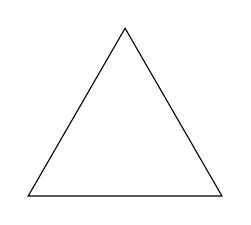
\begin{tikzpicture}
    \draw[Koch curve={order=0,step=70pt/3^(0)}] l-system -- cycle;
  \end{tikzpicture} &   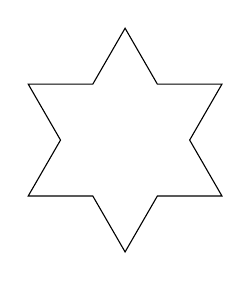
\begin{tikzpicture}
    \draw[Koch curve={order=1,step=70pt/3^(1)}] l-system -- cycle;
  \end{tikzpicture} & 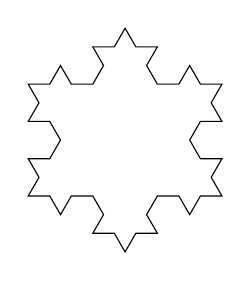
\begin{tikzpicture}
    \draw[Koch curve={order=2,step=70pt/3^(2)}] l-system -- cycle;
  \end{tikzpicture} & 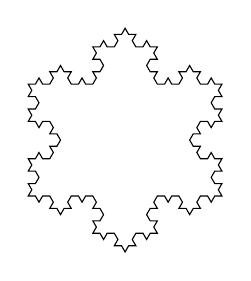
\begin{tikzpicture}
    \draw[Koch curve={order=3,step=70pt/3^(3)}] l-system -- cycle;
  \end{tikzpicture}\tabularnewline
$C_{1}$ & $C_{2}$ & $C_{3}$ & $C_{4}$\tabularnewline
\end{tabular}
\par\end{center}
\medskip{}

In this investigation we consider a \textbf{limit curve} named after
the Swedish mathematician Niels Fabian Helge von Koch (1860-1924).

\medskip{}

To draw von Koch's snowflake we:

\begin{itemize}

\item  start with an equilateral triangle $C_{1}$

\item  divide each side into $3$ equal parts

\item  on each middle part, draw an equilateral triangle

\item  delete the side of the smaller triangle which lies on $C_{1}$

\end{itemize}

\medskip{}

The resulting curve is $C_{2}$. By repeating this process on every
edge of $C_{2}$, we generate $C_{3}$.

\medskip{}

Hence we obtain a sequence of special curves $C_{1},C_{2},C_{3},C_{4},\ldots$
and von Koch's curve is the limiting case when $n$ is infinitely
large.

\medskip{}

Let us investigate the perimeter and area of von Koch's curve.

\medskip{}

\begin{enumerate}

\item \begin{enumerate}[label=(\alph*)]

\item  Find the number of sides of $C_{1}$, $C_{2},C_{3},C_{4}$
and $C_{5}$.

\item  Find the number of sides of the $n\text{th}$ snowflake. 

\end{enumerate}

\end{enumerate}

It is given that $C_{1}$ has perimeter $3$ units. 

\begin{enumerate}[start=2]

\item \begin{enumerate}[label=(\alph*)]

\item  Find the perimeter of $C_{2},C_{3},C_{4}$ and $C_{5}$.

\item  Remembering that von Koch's curve is $C_{n}$, where $n$
is infinitely large, find the perimeter of von Koch's curve.

\end{enumerate}

\item \begin{enumerate}[label=(\alph*)]

\item  Find the areas of $C_{2},C_{3},C_{4}$ and $C_{5}$.

\item  What will be the area within von Koch's snowflake?

\end{enumerate}

\item  Is there anything remarkable about your answers in $1$ and
$2$?

\end{enumerate}
\end{investigation}

\newpage

\section{Applications of AP and GP}

\begin{example}

A frog which is stuck at the bottom of a well is trying to make a
series of vertical upward jumps on the well wall to get out. Its first
jump is $1\,\text{m}$, but because of fatigue and over-exertion,
each subsequent jump is $90\%$ of the distance of the previous jump. However, as the wall is wet and slippery, the frog slips down some distance after every jump is made. It slips down $0.3\,\text{m}$ after its first jump, but because it learns to grip better, each subsequent jump is $0.02\,\text{m}$ less than that of the previous slip such that by the $15\text{th}$ jump, the frog will no longer slip. 

\begin{enumerate}[label=(\alph*)]

\item  Find the total distance covered by $n$ jumps, where $n\leq15$.

\item  Find the total distance covered by the $15\text{th}$ jump
to $5$ significant figures.

\item  How many jumps are needed for the frog to clear the $4\,\text{m}$ mark in the well?

\item  How many jumps are needed for the frog to clear the $6.5\,\text{m}$ mark in the well?

\item  Determine the greatest possible distance the frog is able
to climb.

\end{enumerate}

\Solution

\begin{enumerate}[label=(\alph*)]

\item  
$
\begin{aligned}[t]
\text{Total Distance Covered} & =\text{Total Jumping Distance}-\text{Total Sliding Distance}\\
 & =\frac{1\left(1-0.9^{n}\right)}{1-0.9}-\frac{n}{2}\left[2\left(0.3\right)+\left(n-1\right)\left(-0.02\right)\right]\\
 & =10\left(1-0.9^{n}\right)-\left[0.3n-0.01n^{2}+0.01n\right]\\
 & =10\left(1-0.9^{n}\right)+0.01n^{2}-0.31n
\end{aligned}
$

\item  When $n=15$, 
\begin{align*}
\text{Total Distance Covered} & =10\left(1-0.9^{15}\right)+0.01\left(15\right)^{2}-0.311\left(15\right)\\
 & =5.5411\,\text{m}
\end{align*}

\item  $10\left(1-0.9^{n}\right)+0.01n^{2}-0.31n\geq4$

From GC, $n\geq8.8715\text{ (5 s.f.)}$

Therefore the frog needs $9$ jumps to pass the $4\,\text{m}$ mark.

\item  After the $15\text{th}$ jump, there will be no more sliding.
Subsequent jumps will follow a GP with first term $0.9^{15}$ and
common ratio $0.9$. Hence 
\begin{align*}
\frac{0.9^{15}\left(1-0.9^{n}\right)}{1-0.9} & \geq6.5-5.5411\\
10\left(0.9^{15}\right)\left(1-0.9^{n}\right) & \geq0.9589
\end{align*}

From GC, $n\geq5.9496\text{ (5 s.f.)}$

Therefore, the least value of $n$ is $6$.

$6+15=21$ jumps are needed to pass the $6.5\,\text{m}$ mark.

\item 
$
\begin{aligned}[t]
\text{Greatest Possible Distance} & =\frac{9^{15}}{1-0.9}+5.5411\\
 & =7.60\,\text{m}
\end{aligned}
$

\end{enumerate}

\end{example}

\begin{example}[Financial Mathematics]

A bank has an account for investors. Interest is added to the account
at the end of each year at a fixed rate of $5\%$ of the amount in
the account at the beginning of that year. A man and a woman both
invest money. 

\begin{enumerate}[label=(\alph*)]

\item  The man decides to invest $\$x$ at the beginning of one year
and then a further $\$x$ at the beginning of the second and each
subsequent year. He also decides that he will not draw any money out
of the account, but just leave it, and any interest, to build up.

\begin{enumerate}[label=(\alph*)]

\item  How much will there be in the account at the end of 1 year,
including the interest?

\item  Show that, at the end of $n$ years, when the interest for
the last year has been added, he will have a total of $\$21\left(1.05^{n}-1\right)x$
in his accounts.

\item  After how many complete years will he have, for the first
time, at least $\$12x$ in his accounts?

\end{enumerate}

\item  The woman decides that, to assist her in her everyday expenses,
she will withdraw the interest as soon as it has been added. She invests $\$y$ at the beginning of each year. Show that at the end of $n$ years, she will receive a total of ${\displaystyle \$\frac{1}{40}n\left(n+1\right)y}$ in interest.

\end{enumerate}

\Solution

\begin{enumerate}[label=(\alph*)]

\item 

\begin{enumerate}[label=(\roman*)]

\item  
$
\begin{aligned}[t]
\text{Amount at the end of the 1st year} & =x+0.05x\\
 & =1.05x
\end{aligned}
$

\item \setlength{\extrarowheight}{2pt}%
\begin{tabular}[t]{|>{\centering}p{3cm}|>{\centering}p{4.5cm}|>{\centering}p{4.5cm}|}
\hline 
 & Amount (start of) & Amount (end of)\tabularnewline
\hline 
1st year & $x$ & $1.05x$\tabularnewline
\hline 
2nd year & $1.05x+x$ & $1.05^{2}x+1.05x$\tabularnewline
\hline 
3rd year & $1.05^{2}x+1.05x+x$ & $1.05^{3}x+1.05^{2}x+1.05x$\tabularnewline
\hline 
\end{tabular}

$
\begin{aligned}[t]
\text{Amount at the end of \ensuremath{n} years} & =1.05x+1.05^{2}x+\ldots+1.05^{n}x\\
 & =x\left(1.05+1.05^{2}+\ldots+1.05^{n}\right)\\
 & =x\left[\frac{\left(1.05\right)\left(1.05^{n}-1\right)}{1.05-1}\right]\\
 & =21\left(1.05^{n}-1\right)x\text{ (shown)}
\end{aligned}
$

\item  
$
\begin{aligned}[t]
21\left(1.05^{n}-1\right)x & \geq12x\\
21\left(1.05^{n}-1\right) & \geq12\\
1.05^{n} & \geq\frac{11}{7}\\
n\ln1.05 & \geq\ln\frac{11}{7}\\
n & \geq9.264
\end{aligned}
$

$\therefore\text{Number of complete years}=10$
 

\end{enumerate}

\item 
\begin{minipage}[t]{0.5\textwidth} 
 \setlength{\extrarowheight}{2pt}%
\begin{tabular}[t]{|>{\centering}p{1.5cm}|>{\centering}p{1.4cm}|>{\centering}p{1.5cm}|>{\centering}p{1.5cm}|}
\hline 
 & Amount (start of) & Amount (end of) & Interest earned\tabularnewline
\hline 
1st year & $y$ & $1.05y$ & $0.05y$\tabularnewline
\hline 
2nd year & $y+y$ & $1.05\left(2y\right)$ & $0.05\left(2y\right)$\tabularnewline
\hline 
3rd year & $2y+y$ & $1.05\left(3y\right)$ & $0.05\left(3y\right)$\tabularnewline
\hline 
\end{tabular}
\end{minipage}
\begin{minipage}[t]{0.45\textwidth} 
\vspace{.5cm}
$
\begin{aligned}[t]
\text{Total Interest} & =0.05y+0.05\left(2y\right)+0.05\left(3y\right)+\ldots0.05\left(ny\right)\\
 & =0.05y\left(1+2+3+\ldots+n\right)\\
 & =0.05y\left(\frac{n}{2}\right)\left(1+n\right)
\end{aligned}
$
\end{minipage}

\end{enumerate}

\end{example}

\newpage

\chapter{Summation}

\section{Sigma Notation}

Instead of appearing as a string of terms, $u_{1}+u_{2}+u_{3}+\ldots+u_{n}$ can be written more concisely using \textbf{sigma notation}.
 The symbol $\sum$ is called sigma. It is the equivalent of capital
S in the Greek alphabet.

\begin{tcolorbox}[colback=blue!5, colframe=black,boxrule=.4pt, sharpish corners]

\[
\sum_{r=1}^{n}u_{r}=u_{1}+u_{2}+u_{3}+\ldots+u_{n}
\]

Where 

\begin{itemize}

\item  $r$ is called the \textbf{index of summation}, and is a dummy
variable, i.e. can be replaced with other letters such as $i,j,m,\text{etc.}$
The index of summation has an \textbf{incremental step of 1}.

\item  Beside the sigma is an expression for the \textbf{general
term} of the series.

\item  Below the sigma is the value of $r$ corresponding to the
\textbf{first term} (in this case 1).

\item  Above the sigma is the value of $r$ corresponding to the
\textbf{last term }(in this case $n$).

\end{itemize}

We read it as ``the sum of all numbers of the form $u_{r}$ where
$r=1,2,3,\ldots,$ up to $n$''
\end{tcolorbox}



\begin{example}

Expand and find the sum of:

\begin{tasks}[label=(\alph*),label-width=3.5ex](3)  

\task  ${\displaystyle \sum_{r=1}^{5}r^{2}}$ 

\task  ${\displaystyle \sum_{r=1}^{4}\frac{\left(-1\right)^{r}}{r}}$ 

\task  ${\displaystyle \sum_{r=0}^{4}r!}$ 

\task  ${\displaystyle \sum_{r=2}^{8}\frac{\ln r}{r+1}}$ 

\task  ${\displaystyle \sum_{r=-2}^{3}r^{3}}$ 

\task  ${\displaystyle \sum_{r=1}^{10}5}$ 

\end{tasks}

\Solution

\begin{tasks}[label=(\alph*),label-width=3.5ex](2)  

\task  
$
\begin{aligned}[t]
\sum_{r=1}^{5}r^{2} & =1^{2}+2^{2}+3^{2}+4^{2}+5^{2}\\
 & =55
\end{aligned}
$
 

\task  
$
\begin{aligned}[t]
\sum_{r=1}^{4}\frac{\left(-1\right)^{r}}{r} & =-1+\frac{1}{2}-\frac{1}{3}+\frac{1}{4}\\
 & =-\frac{7}{12}
\end{aligned}
$
 

\task  
$
\begin{aligned}[t]
\sum_{r=0}^{4}r! & =0!+1!+2!+3!+4!\\
 & =34
\end{aligned}
$ 

\task  
$
\begin{aligned}[t]
\sum_{r=2}^{6}\frac{\ln r}{r+1} & =\frac{\ln2}{3}+\frac{\ln3}{4}+\frac{\ln4}{5}+\frac{\ln5}{6}+\frac{\ln6}{7}\\
 & =1.31\text{ (3 s.f.)}
\end{aligned}
$

\task  
$
\begin{aligned}[t]
{\displaystyle \sum_{r=-2}^{3}r^{3}} & =\left(-2\right)^{3}+\left(-1\right)^{3}+\left(0\right)^{3}+1^{3}+2^{3}+3^{3}\\
 & =27
\end{aligned}
$

\task  
$
\begin{aligned}[t]
\sum_{r=1}^{10}5 & =5+5+\ldots+5\\
 & =50
\end{aligned}
$
 
\end{tasks}

\end{example}

\newpage

\section{Writing a Series in $\sum$ Notation}

If we are able to find the general term of a series, we can write
the series in $\sum$ (sigma) notation. For example, we can see that
the general term of the series 
\[
\frac{1}{2}+\frac{1}{4}+\frac{1}{8}+\ldots+\left(\frac{1}{2}\right)^{n-1}+\left(\frac{1}{2}\right)^{n}
\]
 is ${\displaystyle \left(\frac{1}{2}\right)^{r}}$. So, we can write
the series as ${\displaystyle \sum_{r=1}^{n}\left(\frac{1}{2}\right)^{r}}$.

\begin{example}

For each of the following series, write down the $r\text{th}$ term
and express the series using $\sum$ notation.

\setlength{\extrarowheight}{12pt}

\begin{tabular}{|>{\centering}p{7cm}|>{\centering}p{3cm}|>{\centering}p{3cm}|}
\hline 
Series

\medskip{} & $r\text{th}$ term & In $\sum$ notation\tabularnewline
\hline 
${\displaystyle \frac{1}{3}+\frac{1}{9}+\frac{1}{27}+\frac{1}{81}}+\ldots$

\medskip{} &  & \tabularnewline
\hline 
${\displaystyle 1-\frac{1}{2}+\frac{1}{4}-\frac{1}{8}+\ldots+\frac{1}{64}}$

\medskip{} &  & \tabularnewline
\hline 
$1+9+25+49+\ldots+169$

\medskip{} &  & \tabularnewline
\hline 
$1\times2+2\times3+3\times4+\ldots+n\left(n+1\right)$

\medskip{} &  & \tabularnewline
\hline 
\end{tabular}

\bigskip

\Solution

\medskip

\setlength{\extrarowheight}{12pt}

\begin{tabular}{|>{\centering}p{7cm}|>{\centering}p{3cm}|>{\centering}p{3cm}|}
\hline 
Series

\medskip{} & $r\text{th}$ term & In $\sum$ notation\tabularnewline
\hline 
${\displaystyle \frac{1}{3}+\frac{1}{9}+\frac{1}{27}+\frac{1}{81}}+\ldots$

\medskip{} & ${\displaystyle \frac{1}{3^{r}}}$ & ${\displaystyle \sum_{r=1}^{\infty}\frac{1}{3^{r}}}$\tabularnewline
\hline 
${\displaystyle 1-\frac{1}{2}+\frac{1}{4}-\frac{1}{8}+\ldots+\frac{1}{64}}$

\medskip{} & ${\displaystyle \left(-\frac{1}{2}\right)^{r}}$ & ${\displaystyle \sum_{r=0}^{6}\left(-\frac{1}{2}\right)^{r}}$\tabularnewline
\hline 
$1+9+25+49+\ldots+169$

\medskip{} & $\left(2r-1\right)^{2}$ & ${\displaystyle \sum_{r=1}^{7}\left(2r-1\right)^{2}}$\tabularnewline
\hline 
$1\times2+2\times3+3\times4+\ldots+n\left(n+1\right)$

\medskip{} & $r\left(r+1\right)$ & ${\displaystyle \sum_{r=1}^{n}r\left(r+1\right)}$\tabularnewline
\hline 
\end{tabular}

\end{example}

\newpage


\section{Rules of Summation}

\centerline{\begin{minipage}{.7\textwidth} 

\begin{tcolorbox}[colback=blue!5, colframe=black,boxrule=.4pt, sharpish corners]

\begin{tabular}{ll}
Constant Multiple Rule:  & ${\displaystyle \sum_{r=1}^{n}\left(ku_{r}\right)=k\sum_{r=1}^{n}u_{r}}$\tabularnewline
Sum and Difference Rule: & ${\displaystyle \sum_{r=1}^{n}\left(u_{r}\pm v_{r}\right)=\sum_{r=1}^{n}u_{r}\pm\sum_{r=1}^{n}v_{r}}$\tabularnewline
Sum of a Constant: & ${\displaystyle \sum_{r=m}^{n}c=c\left(n-m+1\right)}$\tabularnewline
Difference of the Sum: & ${\displaystyle \sum_{r=m}^{n}u_{r}=\sum_{r=1}^{n}u_{r}-\sum_{r=1}^{m-1}u_{r}}$\tabularnewline
\end{tabular}

\begin{tasks}[style=itemize,label-width=3.5ex](2)  

\task  ${\displaystyle \sum_{r=1}^{n}r=\frac{n\left(n+1\right)}{2}}$

\task  ${\displaystyle \sum_{r=1}^{n}r^{2}=\frac{n\left(n+1\right)\left(2n+1\right)}{6}}$

\task  ${\displaystyle \sum_{r=1}^{n}r^{3}=\frac{n^{2}\left(n+1\right)^{2}}{4}}$

\task  ${\displaystyle \sum_{i=1}^{n}ar^{i-1}=\frac{a\left(1-r^{n}\right)}{1-r}}$ 

\end{tasks}
\end{tcolorbox}

\end{minipage}}

\begin{example}

Evaluate the following sums.

\begin{tasks}[label=(\alph*),label-width=3.5ex](4)  

\task ${\displaystyle \sum_{r=0}^{10}\left(2r+3\right)}$

\task ${\displaystyle \sum_{r=20}^{40}r^{3}}$

\task  ${\displaystyle \sum_{r=1}^{n}\left(3^{r-1}+2r\right)}$

\task  ${\displaystyle \sum_{r=1}^{n-1}\left(r^{2}+2^{r}\right)}$

\end{tasks}

\Solution

\begin{tasks}[label=(\alph*),label-width=3.5ex](2)  

\task*  \begin{minipage}[t]{0.45\textwidth} 

$
\begin{aligned}[t]
\sum_{r=0}^{10}\left(2r+3\right) & =2\sum_{r=0}^{10}r+\sum_{r=0}^{10}3\\
 & =2\sum_{r=1}^{10}r+\left(11\right)\left(3\right)\\
 & =2\left[\frac{1}{2}\left(10\right)\left(11\right)\right]+33\\
 & =110+33=143
\end{aligned}
$

\end{minipage}
\begin{minipage}[t]{0.45\textwidth} 

Alternatively, notice that the series is an arithmetic series with
first term $3$ and common difference $2$.

$
\begin{aligned}[t]
\sum_{r=0}^{10}\left(2r+3\right) & =3+5+7+\ldots+23\\
 & =\frac{11}{2}\left[2\left(3\right)+10\left(2\right)\right]\\
 & =143
\end{aligned}
$

\end{minipage}

\task  
$
\begin{aligned}[t]
\sum_{r=20}^{40}r^{3} & =\sum_{r=1}^{40}r^{3}-\sum_{r=1}^{19}r^{3}\\
 & =\frac{40^{2}\times41^{2}}{4}-\frac{19^{2}\times20^{2}}{4}\\
 & =636300
\end{aligned}
$

\task 
$
\begin{aligned}[t]
\sum_{r=1}^{n}\left(3^{r-1}+2r\right) & =\sum_{r=1}^{n}3^{r-1}+\sum_{r=1}^{n}2r\\
 & =\frac{1\left(3^{n}-1\right)}{3-1}+2\left[\frac{n}{2}\left(n+1\right)\right]\\
 & =\frac{1}{2}\left(3^{n}-1\right)+n\left(n+1\right)
\end{aligned}
$

\task 
$
\begin{aligned}[t]
\sum_{r=1}^{n-1}\left(r^{2}+2^{r}\right) & =\sum_{r=1}^{n-1}r^{2}+\sum_{r=1}^{n-1}2^{r}\\
 & =\frac{\left(n-1\right)\left(n\right)\left(2n-1\right)}{6}+\frac{2\left(2^{n-1}-1\right)}{2-1}\\
 & =\frac{1}{6}\left(n-1\right)\left(n\right)\left(2n-1\right)+2\left(2^{n-1}-1\right)
\end{aligned}
$

\end{tasks}

\end{example}

\newpage

\begin{example}

Under what conditions will the series ${\displaystyle \sum_{r=0}^{\infty}50\left(2x-1\right)^{r-1}}$ converge? 

Find ${\displaystyle \sum_{r=0}^{\infty}50\left(2x-1\right)^{r-1}}$
if $x=0.3$.

\Solution

${\displaystyle \sum_{r=0}^{\infty}50\left(2x-1\right)^{r-1}}$ is
a geometric series with first term $50$ and common ratio $2x-1$.

For the series to converge, $\left|2x-1\right|<1$. 

\begin{align*}
-1 & <2x-1<1\\
-2 & <2x<2\\
-1 & <x<1
\end{align*}

If $x=0.3$, 

\begin{align*}
{\displaystyle \sum_{r=0}^{\infty}50\left(2\left(0.3\right)-1\right)^{r-1}} & =\sum_{r=0}^{\infty}50\left(-0.4\right)^{r-1}\\
 & =\frac{50}{1-\left(-0.4\right)}\\
 & =\frac{250}{7}
\end{align*}

\end{example}


\section{Method of Difference}

The method of difference is used to evaluate sums where the $r\text{th}$
term $u_{r}$ can be expressed as a difference of two (or more) terms,
in such a way that will result in the cancellation of most of the
intermediate terms.

Suppose the general term of a series is $u_{r}=f\left(r\right)-f\left(r-1\right)$,
where $f\left(r\right)$ is an expression in terms of $r$, then

\begin{align*}
\sum_{r=1}^{n}u_{r}= & \sum_{r=1}^{n}\left[f\left(r\right)-f\left(r-1\right)\right]\\
= & \left\{ \:\begin{aligned} & \qquad\bcancel{f\left(1\right)}\quad-\quad f\left(0\right)\\
+ & \qquad\bcancel{f\left(2\right)}\quad-\quad\bcancel{f\left(1\right)}\\
+ & \qquad\bcancel{f\left(3\right)}\quad-\quad\bcancel{f\left(2\right)}\\
+ & \ldots\\
+ & \;\bcancel{f\left(n-1\right)\quad}-\quad\bcancel{f\left(n-2\right)}\\
+ & \hspace{1.8em} f\left(n\right)\quad-\quad\bcancel{f\left(n-1\right)}
\end{aligned}
\right.\\
= & f\left(n\right)-f\left(0\right)
\end{align*}

\newpage

\begin{example}

Express ${\displaystyle \frac{1}{r\left(r+1\right)}}$ in partial
fractions.

Hence prove that ${\displaystyle \frac{1}{1\times2}+\frac{1}{2\times3}+\frac{1}{3\times4}+\ldots+\frac{1}{n\left(n+1\right)}=1-\frac{1}{n+1}}$.

\Solution

Let ${\displaystyle \frac{1}{r\left(r+1\right)}=\frac{A}{r}+\frac{B}{r+1}}$,
where $A$ and $B$ are constants.

Then $1=A\left(r+1\right)+Br$.

Comparing Coefficients, 
\begin{align*}
A+B & =0\tag{1}\\
A= & 1\tag{2}
\end{align*}

Substituting (2) into (1), 

\begin{align*}
1+B & =0\\
B & =-1
\end{align*}

Hence, ${\displaystyle \frac{1}{r\left(r+1\right)}=\frac{1}{r}-\frac{1}{r+1}}$.

\begin{align*}
\frac{1}{1\times2}+\frac{1}{2\times3}+\frac{1}{3\times4}+\ldots+\frac{1}{n\left(n+1\right)}= & \sum_{r=1}^{n}\frac{1}{r\left(r+1\right)}\\
= & \sum_{r=1}^{n}\left(\frac{1}{r}-\frac{1}{r+1}\right)\\
= & \hspace{2em}\quad\frac{1}{1}\qquad-\qquad\frac{1}{2}\\
 & \quad+\quad\frac{1}{2}\qquad-\qquad\frac{1}{3}\\
 & \quad+\quad\frac{1}{3}\qquad-\qquad\frac{1}{4}\\
 & \quad+\quad\ldots\\
 & \quad+\hspace{0.14cm}\frac{1}{n-1}\hspace{0.3cm}-\qquad\frac{1}{n}\\
 & \quad+\hspace{0.3cm}\frac{1}{n}\qquad-\hspace{0.4cm}\frac{1}{n+1}\\
= & 1-\frac{1}{n+1}
\end{align*}

\end{example}

\newpage

\begin{example} 

Given that $f\left(r\right)=\left(r+1\right)!$, find $f\left(r\right)-f\left(r-1\right)$.
Hence find ${\displaystyle \sum_{r=1}^{n}r!\cdot r}$.

\Solution

\begin{align*}
f\left(r\right)-f\left(r-1\right) & =\left(r+1\right)!-r!\\
 & =r!\left(r+1-1\right)\\
 & =r!\cdot r
\end{align*}

\begin{align*}
\sum_{r=1}^{n}r!\cdot r & =\sum_{r=1}^{n}\left[f\left(r\right)-f\left(r-1\right)\right]\\
 & =\hspace{1cm}{f\left(1\right)}\qquad-\qquad f\left(0\right)\\
 & \qquad+\quad{f\left(2\right)}\qquad-\qquad{f\left(1\right)}\\
 & \qquad+\quad{f\left(3\right)}\qquad-\qquad{f\left(2\right)}\\
 & \qquad+\quad\ldots\\
 & \qquad+\quad{f\left(n-1\right)}\hspace{0.3em}-\quad{f\left(n-2\right)}\\
 & \qquad+\quad f\left(n\right)\hspace{0.63cm}-\quad{f\left(n-1\right)}\\
 & =f\left(n\right)-f\left(0\right)\\
 & =\left(n+1\right)!-1
\end{align*}

\end{example}

\begin{example} 

Given than ${\displaystyle \frac{1}{r\left(r^{2}-1\right)}=\frac{1}{2\left(r-1\right)}-\frac{1}{r}+\frac{1}{2\left(r+1\right)}}$,
show that ${\displaystyle \sum_{r=2}^{n}\frac{1}{r\left(r^{2}-1\right)}=\frac{1}{4}+\frac{1}{2\left(n+1\right)}-\frac{1}{2n}}$.

\Solution

\begin{align*}
\sum_{r=2}^{n}\frac{1}{r\left(r^{2}-1\right)} & =\sum_{r=2}^{n}\left(\frac{1}{2\left(r-1\right)}-\frac{1}{r}+\frac{1}{2\left(r+1\right)}\right)\\
 & =\qquad\quad\frac{1}{2\times1}-\frac{1}{2}+\frac{1}{2\times3}\\
 & \qquad+\quad\frac{1}{2\times2}-\frac{1}{3}+\frac{1}{2\times4}\\
 & \qquad+\quad\frac{1}{2\times3}-\frac{1}{4}+\frac{1}{2\times5}\\
 & \qquad+\quad\frac{1}{2\times4}-\frac{1}{5}+\frac{1}{2\times6}\\
 & \qquad+\quad\ldots\\
 & \qquad+\quad\frac{1}{2\left(n-3\right)}-\frac{1}{n-2}+\frac{1}{2\left(n-1\right)}\\
 & \qquad+\quad\frac{1}{2\left(n-2\right)}-\frac{1}{n-1}+\frac{1}{2n}\\
 & \qquad+\quad\frac{1}{2\left(n-1\right)}-\frac{1}{n}+\frac{1}{2\left(n+1\right)}\\
 & =\frac{1}{2}-\frac{1}{2}+\frac{1}{4}+\frac{1}{2n}-\frac{1}{n}+\frac{1}{2\left(n+1\right)}\\
 & =\frac{1}{4}+\frac{1}{2\left(n+1\right)}-\frac{1}{2n}\text{ (Shown)}
\end{align*}

\end{example}

\newpage{}

\section{Convergence of an Infinite Sequence}

Consider the following infinite sequence

\[
u_{n}=\frac{n}{n+1},\:n\in\N\text{ and }n\geq1
\]

Writing the sequence out and plotting its graph, 

\begin{minipage}{0.5\textwidth} 

\[
\frac{1}{2},\:\frac{2}{3}\:,\frac{3}{4}\:,\ldots\:,\:\frac{97}{98},\:\frac{98}{99},\:\frac{99}{100}\:,\ldots\:,\:\frac{n}{n+1},\:\ldots
\]

\end{minipage}
\begin{minipage}{0.5\textwidth} 
\begin{center}
\includegraphics[width=6cm,valign=t]{\string"lib/Graphics/CovergentSequence\string".png}
\par\end{center}

\end{minipage}

We notice that the terms of the sequence ${\displaystyle u_{n}=\frac{n}{n+1}}$
is approaching $1$ as $n$ becomes large but it never equals to $1$.

We say that the terms of the sequence tend to the limit $1$ as $n$
tends to infinity. We indicate this by writing

\[
\lim_{n\to\infty}\left(\frac{n}{n+1}\right)=1
\]

This sequence is \textbf{convergent}.

\begin{tcolorbox}[colback=blue!5, colframe=black,boxrule=.4pt, sharpish corners]

If the terms of the sequence $u_{n}$ converge to a limit $L$ as
$n$ tends to infinity, we write

\[
\lim_{x\to\infty}\left(u_{n}\right)=L\qquad\text{ or }\qquad\text{As }\;n\to\infty,\;u_{n}\to L
\]

Otherwise, the sequence diverges.
\end{tcolorbox}

\begin{example}

Find the limit of each sequence (if it exists) as $n$ approaches
infinity.

\begin{tasks}[label=(\alph*),label-width=3.5ex](3)  

\task  ${\displaystyle u_{n}=\frac{5n+1}{n}}$

\task  ${\displaystyle u_{n}=\frac{3n^{2}-n+1}{n^{2}+1}}$

\task  $u_{n}=2^{r}$

\end{tasks}

\Solution

\begin{tasks}[label=(\alph*),label-width=3.5ex](2)  

\task  
$
\begin{aligned}[t]
\lim_{x\to\infty}u_{n} & =\lim_{x\to\infty}\frac{5n+1}{n}\\
 & =\lim_{x\to\infty}\left(5+\frac{1}{n}\right)\\
 & =5+\lim_{n\to\infty}\left(\frac{1}{n}\right)\\
 & =5
\end{aligned}
$

\task  
$
\begin{aligned}[t]
\lim_{x\to\infty}u_{n} & =\lim_{x\to\infty}\frac{3n^{2}-n+1}{n^{2}+1}\\
 & =\lim_{x\to\infty}\frac{3-\frac{1}{n}+\frac{1}{n^{2}}}{1+\frac{1}{n^{2}}}\\
 & =3
\end{aligned}
$

\task* $u_{n}=2^{r}=2+4+8+16+\ldots$

As $n\to\infty$, $2^{r}\to\infty$

Thus, the sequence diverges and the limit of the sequence does not
exist.

\end{tasks}

\end{example}

\section{Convergence of an Infinite Series (Sum to Infinity)}

\begin{tcolorbox}[colback=blue!5, colframe=black,boxrule=.4pt, sharpish corners]

If a series $S_{n}$ converges to a limit $L$ as $n$ tends to infinity,
we write

\[
\lim_{x\to\infty}S_{n}=\sum_{r=1}^{\infty}u_{r}=\lim_{n\to\infty}\sum_{r=1}^{n}u_{r}=L
\]

Otherwise, the series diverges.
\end{tcolorbox}

\begin{example}

Determine whether the series in examples \textsf{5.5}, \textsf{5.6} and \textsf{5.7} are convergent and state the sum to infinity (if it exists).

\Solution

\textsf{Example 5.5}

\[
\sum_{r=1}^{n}\frac{1}{r\left(r+1\right)}=1-\frac{1}{n+1}
\]

\begin{align*}
\sum_{r=1}^{\infty}\frac{1}{r\left(r+1\right)} & =\lim_{n\to\infty}\left(1-\frac{1}{n+1}\right)\\
 & =1
\end{align*}

Since the series tends to a limit of $1$ as $n\to\infty$, the series
is \textbf{convergent}.

\bigskip

\textsf{Example 5.6}

\[
\sum_{r=1}^{n}r!\cdot r=\left(n+1\right)!-1
\]

As $n\to\infty$, $\left(n+1\right)!-1\to\infty$. Thus the series
is \textbf{not convergent}.

\bigskip

\textsf{Example 5.7}

\[
\sum_{r=2}^{n}\frac{1}{r\left(r^{2}-1\right)}=\frac{1}{4}+\frac{1}{2\left(n+1\right)}-\frac{1}{2n}
\]

\begin{align*}
{\displaystyle \sum_{r=2}^{\infty}\frac{1}{r\left(r^{2}-1\right)}} & =\lim_{n\to\infty}\left(\frac{1}{4}+\frac{1}{2\left(n+1\right)}-\frac{1}{2n}\right)\\
 & =\frac{1}{4}
\end{align*}

Since the series tends to a limit of ${\displaystyle \frac{1}{4}}$
as $n\to\infty$, the series is \textbf{convergent}.

\end{example}
% End document
\end{document}
